%Hayden Thesis, table 1.4, p24

\documentclass{article}
\usepackage{multirow}
\usepackage{subcaption}
\usepackage[utf8x]{inputenc} 
\usepackage{graphicx}
\usepackage{amssymb}
\usepackage{amsmath}
\usepackage{bm}
\usepackage{physics}
\usepackage{cite}
\usepackage{titlesec}
\usepackage{setspace}
\usepackage[margin=1.0in]{geometry}
%For numbering%%%
\usepackage{etoolbox}
\makeatletter
\patchcmd{\ttlh@hang}{\parindent\z@}{\parindent\z@\leavevmode}{}{}
\patchcmd{\ttlh@hang}{\noindent}{}{}{}
\makeatother
%%%%%%%%%%%%%%%%%
\title{Search For New Physics at ATLAS}
\author{Michael Hayes}
\date{Supervisor: Dr Tracey Berry}
%add section numbering
\titleformat{\section}[block]
  {\fontsize{17.28}{18}\bfseries\sffamily\filcenter\raggedright}
  {\thesection}
  {1em}
  {}
\titleformat{\subsection}[hang]
  {\fontsize{14}{15}\bfseries\sffamily\filcenter\raggedright}
  {\thesubsection}
  {1em}
  {}
\titleformat{\subsubsection}[hang]
  {\fontsize{12}{14}\bfseries\sffamily\filcenter\raggedright}
  {\thesubsubsection}
  {1em}
  {}

\begin{document}
\maketitle
\large
\onehalfspacing
\section*{Abstract}
\addtocounter{section}{1}
The $Z'$ is a hypothetical particle predicted by extensions to the Standard Model such as $E_6$ GUT models and the Sequential Standard Model (SSM). This paper analyses the search for the $Z'$ by looking at simulated Monte Carlo events.

\clearpage
\normalsize
\tableofcontents
\clearpage
\large
\section{Introduction}%%%%%%%%%%%%%%%%%%%%%%%%%%%%%%%%%%%%%%%%%%%%%%%%%%%%%%
\label{sec:Introduction}
The Standard Model, or SM, is the product of the advances in theoretical and experimental particle physics over the course of the past century. While it has been incredibly successful in explaining experimental results, it is far from a complete theory of nature. The Standard Model is has over 22 free parameters which are fixed through experimental observations without any underlying reasoning why, which is view as a theoretically unappealing property. It is also unable to be reconciled with gravity, and does not offer any realistic dark matter candidates. 

However, there are a number of possible extensions to the Standard Model that are able to address these limitations. Grand Unified Theories (or GUTs), for example, continue the method of invoking gauge invariance that has been the foundation of the Standard Model. These involve embedding the gauge groups of the Standard Model ($SU(3)_C \otimes SU(2)_L \otimes U(1)$) into a single, larger gauge group such as $SO(10)$ or $E_6$. The introduction of new fields to maintain the invariance of the Lagrangian results in new gauge bosons, allowing the new physics to emerge in this theory.

Large Hadron Collider, which started taking data in 2008, is a synchrotron that collides protons together at a centre of mass energy of up to $\sqrt{s} = 14\,$TeV and is currently the most powerful particle accelerator on the planet. This review data will utilise data collected at the ATLAS detector, one of the two general purpose detectors at the LHC, to search for the the existance of the $Z'$ boson.

In particular, the search will focus on looking for an excess in dilepton final states in the TeV range. Dilepton final states are most often described by a charged lepton and its corresponding antiparticle, such as $e^+e^-$ or $\mu^+\mu^-$ pairs. The electron-positron pair final state is of particular interest in this paper. While a $Z'$ could feasibly decay in a number of possible ways such as $q\overline{q}$, the dilepton final states are attractive from an experimental standpoint as they are simpler to resolve. Electrons and positrons are stable, unlike mesons which decay into a number of possible final state particles, some of which cannot be detected such as neutrinos. This review data will utilise Monte Carlo data of simulated events at the ATLAS detector and analyse these in ROOT \cite{ROOT} in order to optimise the search.

Section \ref{sec:TheoreticalMotication} introduces the theoretical motivation behind looking beyond the Standard Model and the search for a $Z'$ boson. Section \ref{sec:ATLAS} gives an overview of the different aspects of the ATLAS detector and how particles are identified, as well as the trigger system at the detector. In Section \ref{sec:Study}, the search for the $Z'$ boson is outlined, including the main background the experiment is subject to and the cuts applied. Section \ref{sec:MonteCarloSimulatedAnalysis} covers an analysis of simulated $Z'$ events and how this can be used to improve the search.

\section{Theoretical Motivation}%%%%%%%%%%%%%%%%%%%%%%%%%%%%%%%%%%%%%%%%%%%%
\label{sec:TheoreticalMotication}

The Standard Model, or SM, represents the signficant advances in theoretical and experimental advances over the course of the past half-century. The SM is composed of three distinct sections- two spin $\frac{1}{2}$ families, leptons and quarks, collectively known as fermions, and a family of spin 1 gauge bosons which act as ``force carriers'' and mediate the interactions between particles. In 2012, the newest addition to the Standard Model was discovered. This was the spin 0 Higgs boson, which had been predicted some decades earlier and was a fundamental component of how the gauge bosons, and the fermions, could gain mass by the process of spontaneous symmetry breaking. 

One of the major cornerstones of the theoretical basis behind the Standard Model has been \textit{gauge invariance}. Gauge invariance can be viewed as being analagous to the principle of general covariance; that is, the underlying physical laws of a theory are not dependant dependant on the coordinate system used to describe them, but rather are invariant under the transformations between differentiable coordinate systems. Similarly, gauge invariance works on the basis of applying a \textit{gauge transformation} to a system, the transformation being described by the mathematics of group theory. 
While the Standard Model has been remarkably successful in explaining experimental phenomena, and there are currently no significiant disagreements with experimental observations, it is not viewed as a fundamental theory of nature. It is at present unable to incorporate one of the four fundamental forces of nature- gravity. The two are often said to be ``fundamentally incompatible''.

At the comparatively low energies acheivable at the LHC, the effect is far weaker than can be measured, and such the results of the Standard Model are still very  consistent with experiments. At much higher energies approaching the Planck scale, the impact of gravity cannot be neglected- this is the scale at which the Standard Model is predicted to break down. Therefore, the Standard Model can be viewed as an effective ``low energy approximation'' of nature, analagous to how the equations of classical mechanics in the regime $v<<c$ and can be retrieved from the Taylor expansion of the equations of special relativity.

In addition, the Standard Model has 22 free parameters are fixed by experimental results; there is no underlying reason for the values these parameters take, which is often seen as a theoretically unsatisfying property. The Standard Model also cannot account for dark matter or neutrino oscillations, and is not able to explain the matter-antimatter asymmetry in the universe. It is therefore hoped that an extension can be found that would solve the questions left unanswered by the Standard Model. 

There are a number of possible extensions to the Standard Model that can potentially solve a number of these issues, each providing varying predictions and theoretical frameworks, but none are currently supported by experimental evidence. Many of these extensions, such as Grand Unified Theories, or GUTs, involve the addition of extra gauge groups or embedding the Standard Model symmetries in a single larger gauge group.

Some of the most theoretically appealing models motivating this paper are $Z$' models based on the  $E_6$ gauge group. These GUT could break down via the patterns \cite{ExtraGaugeBosonsE6}
\begin{equation}
E_{6} \rightarrow SO(10) \otimes U(1)_\Psi \rightarrow SU(5)\otimes U(1)_\chi \otimes U(1)_\Psi
\end{equation}
or 
\begin{equation}
E_{6} \rightarrow SO(10) \otimes U(1)_\Psi \rightarrow SU(4) \otimes SU(2)_L \otimes SU(2)_R \otimes U(1)_\Psi,
\end{equation}

for example. A consequence of these extra gauge groups are additional gauge bosons, the most important to this paper being the $Z'$ bosons. If there does indeed exists a $Z'$ field, the states $Z$ and $Z'$ would be formed by a linear combination of mass eigenstates $Z_1$ and $Z_2$ \cite{ColliderPhysics}

\begin{equation}
\begin{split}
Z & = \cos\theta Z_1 - \sin\theta Z_2 \\
Z & = \sin\theta Z_1 + \cos\theta Z_2. \\
\end{split}
\end{equation}

This is analagous to how the photon and Standard Model Z boson are made up of a linear combination of the $W^{0}_\mu$ and $B_\mu$ bosons from the electroweak group $SU(2)_L \otimes U(1)_Y$. The $Z'$ mass is predicted to be on the order of $1\,$TeV. This is within range of the LHC, unlike other GUT bosons such as the X and Y meaning that direct searches for GUT particles is possible rather than relying on indirect searches such as proton decay.

\section{ATLAS Detector}%%%%%%%%%%%%%%%%%%%%%%%%%%%%%%%%%%%%%%%%%%%%%%%%%%%%
\label{sec:ATLAS}

The Large Hadron Collider, or LHC, is the world's highest energy particle accelerator, with a circumference of $27\,$km and max attainable centre of mass energy of $13\,$TeV. 
ATLAS (A Toroidal LHC ApparatuS) \cite{ATLAS}, as seen in Figure (\ref{fig:ATLASDiagram}), is one of the two general purpose detectors at the LHC, the other being CMS (Compact Muon Solenoid). The ATLAS detector is made up of several distinct components, each with a different task. As it is important to understand how ATLAS works when analysing the data taken from the detector, this section will give an overview of how ATLAS functions and the general principles behind it. Section \ref{sec:ATLAS_DetectorSchematics} covers the main components of the ATLAS detector and how they function.

\begin{figure}[h]
    \centering
    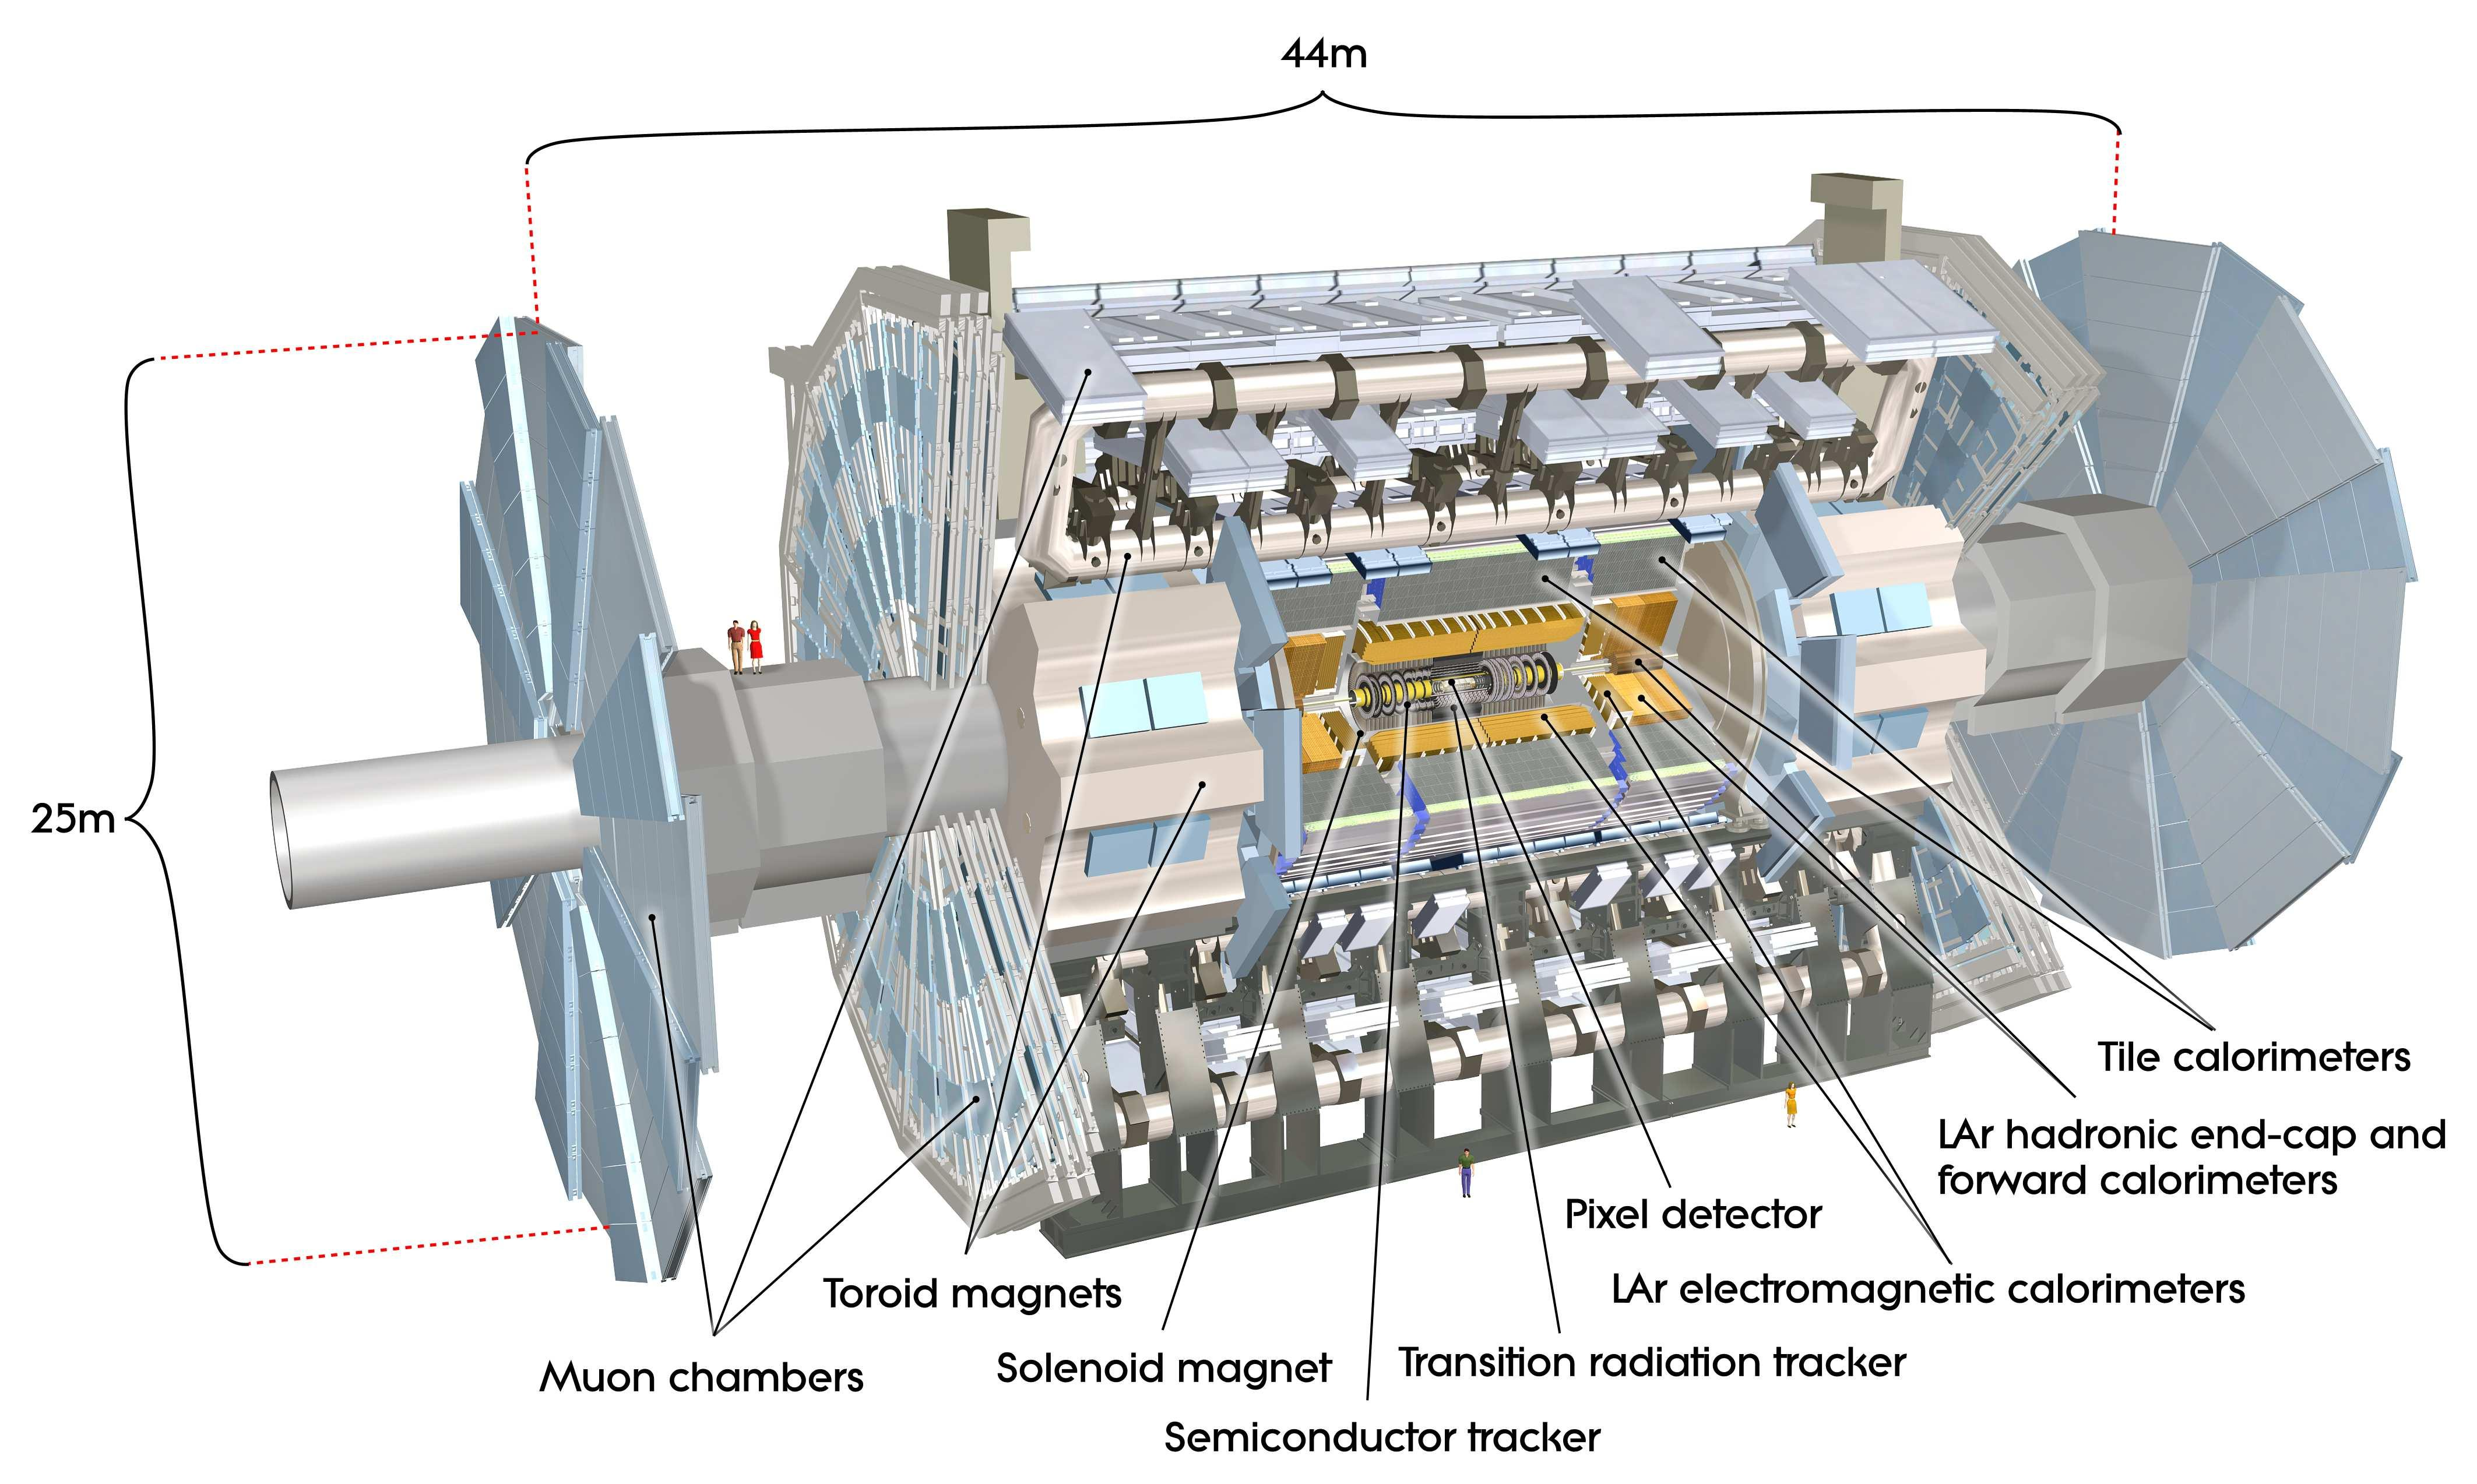
\includegraphics[scale=0.075]{images/AtlasDetector.jpg}
    \caption{ Diagram of the ATLAS detector \cite{ATLASReview}. \label{fig:ATLASDiagram} }
\end{figure}

\subsection{Detector Schematics}
\label{sec:ATLAS_DetectorSchematics}

The ATLAS detector is described in terms of a right handed coordinate system with an orgin at the nominal interaction point in the centre of the detector. The positive $x$ direction is defined as pointing from the nominal interaction point to the centre of the LHC ring, and the positive $y$ direction being up. The $z$ axis is parallel to the beam direction, with the azimuthal angle $\phi$ measured around the $z$ beam axis, and the polar angle $\theta$ in the $x-y$ plane. The pseudorapidity is defined as $\eta = -\ln\tan(\theta/2)$ \cite{ATLASReview}.

The ATLAS detector is composed of an Inner Detector (ID) tracking system composed of pixel/SCT and TRT detectors surrounded by a solenoidal magnet providing a magnetic field of $2\,$T, and electromagnetic and hadronic sampling calorimeters in the outer regions. A calorimeter is designed to measure the energy of an incident particle by completely absorbing its initial energy and then analysing the impact of this absorption.

\begin{figure}[h]
    \centering
    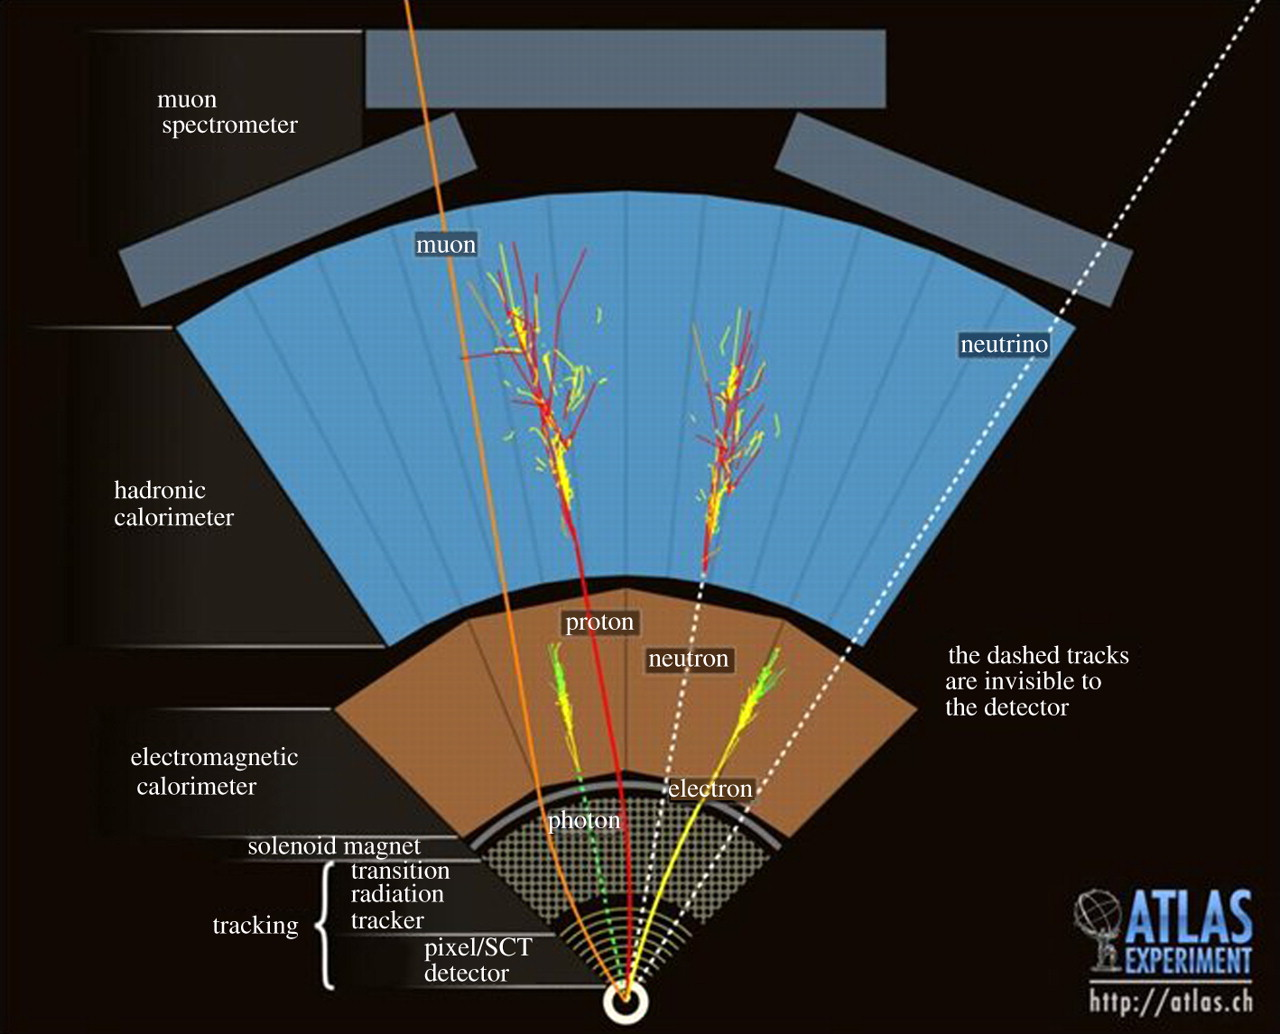
\includegraphics[scale=0.25]{images/DetectorCrossSection.jpg}
    \caption{ Transverse view of the ATLAS detector \cite{PhysicsRequirementsATLAS}. \label{fig:DetectorCrossSection} }
\end{figure}

\begin{table}[h!t]
%http://www.nikhef.nl/pub/experiments/atlas/daq/Dankers/chapter_02.pdf
\label{table:ATLASSpec}
\centering
\caption{Dimensions of Atlas sub detectors. x- integrated in end-cap }
\begin{tabular}{ |c|c|c|c| } 
\hline
component&radius[m]&length[n]&$\eta$-coverage\\
\hline
 barrel muon spectrometer & 11 & 26 & $|\eta|<1.4$\\
 end-cap muon spectrometer & 11 & 2.8 & $1.1<|\eta|<2.8$\\
 barrel hadronic calorimeter & 4.25 & 12.2 & $|\eta|<1.0$\\
 end-cap hardronic calorimeter & 2.25 & 2.25 & $1.5<|\eta|<3.2$\\
 barrel em-calorimeter & 2.25 & 6.42 & $|\eta|<1.4$\\
 end-cap em-calorimeter & 2.25 & 0.63 & $1.4<|\eta|<3.2$\\
 forward/backward calorimeter & x & x & $3.1<|\eta|<4.9$\\
 barrel + end-cap inner detector & 1.15 & 6.8 & $|\eta|<2.4$\\
 \hline
\end{tabular}
\end{table}

\subsubsection{Inner Detector}
\label{sec:ATLAS_DetectorSchematics_ID}
The ATLAS Inner Detector is used to provide accurate position resolution of charged particles as they pass through. 

%%%%%%%%%%%%%%%%%%%%%%%%%%%%%%%%%%%%%%%%%%%%%%%%%%%%%%%%%%%%%%%
The innermost part of ATLAS consists of three layers of silicon pixels surrounding the beampipe, forming over 80 million radiation hardened pixels. \cite{ATLASPixelDetector}. The pixel detector is made up of around 1,700 modules. Each module is a silicon sensor approximately $2\times6\,\rm{cm}^2$ in dimension, which is divided subdivided into around 47,000 pixels individually connected to 16 front end chips. The smallest pixel unit is around $50\mu\,$m by $400\mu\,$m. This provides a very high position resolution close to the interaction point. 
%%%%%%%%%%%%%%%%%%%%%%%%%%%%%%%%%%%%%%%%%%%%%%%%%%%%%%%%%%%%%%%
The middle part of inner detector is a Semi-Conductor Tracker made (SCT) made of silicon microstrip layers\cite{ATLASReview},  providing a high granularity at larger radii. The output of this subdetector component is binary, providing whether it has been hit or not as opposed to the number of hits at that layer.

The outer layer of inner detector is comprised of a Transition Radiation Tracker (TRT), which are straw tube trackers covering up to a psuedorapidity of $|\eta|<1$. These are drift tubes that are able to provide good performance at high occupancy (the number of particles passing through a detector cell per event) and high counting rate. 

A solenoid magnet surrounding the ID provides a magnetic field of $2\,$T, exerting a force on any charged particle as it moves through the field. This allows the sign of the particle's charge and the momentum/charge ratio by observing the radius of curvature through the equation 
\begin{equation} 
r = \frac{\underline{p}}{\underline{B}q}. 
\end{equation}

\subsubsection{Presampler}
\label{sec:ATLAS_DetectorSchematics_Presampler}

As the particles generated in an event pass through the detector, they lose energy through a variety of processes such as ionisation and nuclear interactions.
As the material in front of the electromagnetic calorimeter amounts to around $1.5X_0$ on average, the barrel and encap calorimeters are accompanied by a presampler detector that covers a pseudorapidity of up to $|\eta| = 1.8$ \cite{EMCParticleIdentification}. The presampler has a thickness of the order of $X_0$, and is designed to estimate the energy lost upstream of the calorimeters, especially in the cryostatm and magnet. This is done on an event by event basis, and is required for obtaining accurate information about the initial energy of the final state particles.

\subsubsection{Electromagnetic Calorimeter}
\label{sec:ATLAS_DetectorSchematics_ECAL}

The energy of a photon or electron produced in the proton-proton collision is measured by analysing the electromagnetic shower produced as the particle passes through the EM calorimeter. 

At energies above $100\,$MeV, the energy loss of a photon passing through a medium is dominated by electron-positron pair production, while electrons lose their energies almost exclusively from bremmstrahlung \cite{RPP}. 
Bremmstrahlung, or `braking radiation', is the electromagnetic radiation that is emmitted when a charged particle is decelerated as it is deflected by another charged particle, such as an electron scattering off a nucleus in the medium it is travelling through. This causes the emission of a photon, which can undergo $e^+e^-$ pair production. These produced electrons can, in turn, lose energy via bremmstrahlung, continuing until the particle energy is below some critical energy $E_c$. This is the energy scale at which bremmstrahlung is no longer the dominant but is instead surpassed by ionisation, and can be approximated by 

As ionisation is now the dominant process for electrons, these particles will stop within a radiation length. However, photons of the same energy are able to continue much further. Therefore, to absorb the majority of bremsstrahlung photons around 7-9 additional radiation lengths of material is required. These `soft' photons escaping the calorimeter are the main cause of energy leakage.

As will be seen in the next section, hadrons are also capable of producing showers of particles through strong interactions. It is important, therefore, to be confident that the shower is due to electromagnetic interactions
The development of em and hadronic showers is dependant on the radiation length and nuclear interaction length respectively. At an atomic number of 82, such as for lead used in as the passive layers in the electromagnetic calorimeter, the nuclear interation length is around 30 times larger than that of the radiation length. Therefore, any shower produced in the electromagnetic calorimeter will be caused by electrons or photons rather than hadrons.

As opposed to a homogenous calorimeter, which uses its entire volume of a material such as NaI or lead glass to detect energy loss of an incident particle, the EMC at ATLAS uses sampling calorimeters formed of layers of lead absorbing plates surrounded by steel plates to provide mechanical strength, interspaced with liquid argonn (LAr) sampling detectors to measure the shower at this point. The advantage of a sampling detector is that a dense material can be used in the absorbing regions with a short radiation length to create a large shower within a short distance with a few sampling layers at various points in the shower evolution. This means the calorimeter is able to be more compact and is cheaper compared to a homogenous detector. 
The EM calorimeter covers a pseudorapidity range of $|\eta|<3.2$ throughout the entire azimuthal angle. Both the barrel and endcap regions have three layers of liquid argon detectors, located at a depth of $3X_0$, $6X_0$ and $16X_0$ \cite{ATLASCalorimetry}. The total thickness of the calorimeter is more than $22X_0$ in the barrel and more than $24X_0$ in the endcap.

\subsubsection{Hadronic Calorimeter}
\label{sec:ATLAS_DetectorSchematics_HCAL}

%https://www.physics.utoronto.ca/~krieger/procs/Krieger_NSS05_Proc.pdf
Hadronic showers, while analagous to their electromagnetic counterparts, are much more complicated due to the number of different processes that may occur, some of which meaning that parts of the hadronic showers are electron cascades. Given that the nuclear interaction length is larger than the radiation length, hadronic calorimeters are required to be significantly larger than electromagnetic calorimeters to fully absorb the energy of an incident particle.

As a high energy hadron passes through a block of matter, it may ionise the medium in a manner similar to a muon. However, at some point the hadron may interact strongly with a nucleus in the medium; this could cause new particles to be produced or the identity of the hadron to change. The nucleus it interacts with could also be affected, potentially losing some of its nucleons through spallation or decaying from an excited state through photon emission. Some of the hadrons produced in a shower, such a $\pi^0$, decay electromagnetically through decay channels such as $\pi^0\rightarrow\gamma\gamma$. These decay products, unlike the hadrons, are able to produce an electron cascade, meaning that hadron showers are often composed of an element of an electromagnetic shower. On average, around a third of the mesons produced in the first generation of nuclear interactions are $\pi^0$s \cite{CalorimetryWigmans}. The remaining hadrons may continue to produce $\pi^0$s in the following interactions provided they are energetic enough. Unlike the electromagnetic showers, in which an electron may produce a photon which can pair produce an electron positron pair, the production of a $\pi^0$ by a meson is not a reversible process. For a more energetic incident hadron, more $\pi^0$s can be produced in the later interactions. This means that the proportion of the initial energy contained in $\pi^0$s, and hence the proportion of the total energy lost through electromagnetic showers gradually increases with the incident particle energy.

Unlike with photons and electrons, where all of the initial energy is eventually used to ionise the surrounding medium and provide a measurable signal, one of the consequences of the strong interaction being involved in hadronic showers is that some of the energy dissipated in the medium is fundamentally unmeasurable. Certain particles, such as muons or neutrinos that could be produced in meson decay, interact through neither the strong force nor produce electromagnetic showers, and so are able to carry away a fraction of energy from the calorimeter. The ratio of visible energy to total incident energy varies due to the incident particle as well as fluctuations in the number of charged to neutral pions, producing a larger uncertainty associated with the measured energy of the incident particle. While this can be compensated with certain methods such as weighting the output of individual counters, the overall resolution of a hadronic calorimeter is generally worse than that of an electromagnetic calorimeter.

The hadronic calorimeter at ATLAS works on a similar process to the EM calorimeter. In the pseudorapidity range $|\eta|<1.6$, the HCAL is composed of an iron scintillating tile detector (TileCal) \cite{ATLASCalorimetry}. It uses iron plates as an absorber and plastic scintillating tiles as the active material. Scintillation light in the tiles is transmitted by wavelength shifting fibres to photomultiplier tubes (PMTs). The total thickness of the calorimeter is chosen as to contain as much of the shower as possible, reducing the background in the muon spectrometer to acceptable levels. 

For $|\eta|>1.6$ the hadronic calorimeter is an LAr calorimeter in between copper plate absorbers. While the process is mainly the same as for the electromagnetic calorimeter, it is not formed in an accordian shape.

\subsubsection{Muon Spectrometer}
\label{sec:ATLAS_DetectorSchematics_Muon}

The muon is one of the two particles, the other being the neutrino, that is able to penetrate beyond the hadronic calorimeter, as they do not emit either a hadronic or electromagnetic shower. Instead, the muon leaves a charged track in these subdetectors. The role of the muon spectrometer is to provide a high precision measurement of the energy and momenta of muons as they pass through, as they are often important in rare processes and contribute to the overall energy resolution of the detector.

The muon spectromer is somewhat similar to the inner detector in that it is centered around measuring the momentum of particles through the radius of curvature as the particle is deflected in the field of a superconducting magnet. In order to increase the precision of the momentum measurement the subdetector is required to be large enough to accurately determine the radius of the muon's curvature, with 1200 Monitered Drift Tubes and multiwire proportional counters located between a radius of $4.25\,$m out to the edge of the detector at $11\,$m \cite{ATLASMuonSpectrometer}. The spectrometer is able to measure the momentum of $100\,$GeV muons with an accuracy of $3\%$ and $1\,$TeV muons with an accuracy of $10\%$.

\subsection{Trigger System}
\label{sec:ATLAS_Trigger}

The LHC has an event rate on the order of $10^7\,$Hz, meaning that a large number of events occur every second. Each event, once compressed, requires around $1.5\,$MB of memory; recording all events would require an enormous amount of memory, and significant effort is put into filtering out as many uninteresting events as possible before writing to memory for offline analysis.

\begin{figure}[h]
    \centering
    \includegraphics[scale=0.6]{images/TDAQ.png}
    \caption{ Diagram showing the different layers of the ATLAS trigger system as it filters out events. The event rates at different parts in the process are shown.\label{fig:TDAQ} }
\end{figure}

This is the job of the trigger system, which at ATLAS is divided into 3 seperate parts, these being Level 1, Level 2 and Event Filtering, denoted as `L1',`L2' and `EF' respectively.  Each level refines the decision made at the previous level through applying additional information and criteria. The L1 trigger is hardware based, while L2 and EF are software based and known together as the High Level Trigger, or HLT. The ATLAS trigger system is visualised in Figure \ref{fig:TDAQ}.

The L1 trigger uses the lower latencies of the hardware and identifies regions of interest that may potentially contain interesting events such as muons or electrons with high transverse momenta or missing energy. As the Level 1 trigger is required to make a decision in around $2.5\,\mu$s, only certain parts of the detector are used, with the inner detector information not being used due to time constraints. The L1 trigger reduces the event rate to around $70\,$kHz. The coordinates $\eta$ and $\phi$ of the region of interest are passed on to the next level.

Using the data provided by the L1 trigger, the L2 level requests all relevant information for the specified region of interest including the inner detector. The L2 trigger level is able to distinguish electrons and photons from the existance of a track in the inner detector leading to the region of interest in the ECAL. Next, by identifying clusters in the calorimeters, the L2 trigger is able to make its decision by implementing algorithms based on the shower shape and track cluster matching. By doing this, the second trigger level is able to check if the region of interest exists when analysed at a higher resolution.

The event filter functions largely in the same way as L2, however implements a full reconstruction of the event, applying more stringent selection criteria to reduce the rate of events saved to permanent storage to a few hundred Hz.

The trigger that will be initially used in this paper is  EF\_g35\_loose\_g25\_loose.

The name of the trigger indicates the requirements for an event to pass it; in this case, `EF' indicates it is an Event Filter level trigger. A letter followed by a number indicates the type of particle and its required energy threshold; here `g' represents a photon, with 35  being the required energy threshold in GeV. Next, `loose' refers to the trigger requiring the particle to pass the loose selection criteria, which is described in Section \ref{sec:cuts_selection}. Therefore, the overall requirement of the trigger is for two photons, one at an energy above $35\,$GeV and one above $25\,$GeV, both having to pass the loose selection criteria before the event is triggered. A photon trigger is used here as the photon and electron triggers are very similar except for the electron triggers including tracking requirements.

\section{Study}
\label{sec:Study}

Fundamentally, in the analysis of the data from the experiment one is looking at the number of events satisfying a set of criteria as a function of the energy of that event. The number of events observed, $n$, is equal to the sum of the background events $b$, and the process that one is looking for, the signal $s$. The value obtained is $n$ is compared to the null hypothesis, which postulates an expected background $b_{expected}$ and no phenomena causing any signal events.

The $p\rm{-value}$ is the probability of observing $n_{obs}$ or more particles under the null hypothesis, that is the probability of observing a result equivalent to the observation made or more contradictory of the null hypothesis. Mathematically, this is expressed as

\begin{equation}
p\rm{-value} = P(n	\geq n_{obs}; b = b_{expected}, s=0).
\end{equation}

The null hypothesis is usually denoted as $H_0$, while the hypothesis that there is some new process contributing to the number of observed events is the signal hypothesis $H_1$.

If this is sufficiently small, the null hypothesis is rejected and a discovery is announced. In high energy physics, this boundary is usually at a $p\rm{-value}$ of $2.9\times10^{-7}$, which corresponds to the probability of quantity following a Poisson distribution being $5\sigma$ from the expectation value.

\subsection{Previous Searches for the $Z'$ and Current Experimental Limits}%%%%%%%%%%%%%%%%%%%%%%%%%%%%%%%

The $Z'$ has been the focus of a number of searches at LEP and the LHC, and these experiments have previously set limits on the mass at which various $Z'$ bosons could exist. The experiment at CMS in 2015 set the lower limits on the $Z_{\rm{SSM}}'$ as $2.90\,$TeV and the superstring $Z_{\Psi}'$ at $2.57\,$TeV \cite{CMSDileptonSearch}. 

\subsection{Main Backgrounds}%%%%%%%%%%%%%%%%%%%%%%

One of the main obstacles facing searches for potentially rare events at the LHC is that the background that may easily drown out any interesting signals if not accounted for. In an experiment, each type of background event can be described as being either reducible or irreducible in nature. Reducible background events, as the name suggests, are events whose frequency can be reduced or cut out entirely through applying certain cuts. These include jets that fake electron signals or top-antitop events which can decay to pair of electrons. Irreducible background events, on the other hand, are those that are, for all intents and purposes, fundamentally indistinguishable from the signal events that are being looked for. 

\begin{figure}[h]
    \centering
    \begin{subfigure}{.25\textwidth}
        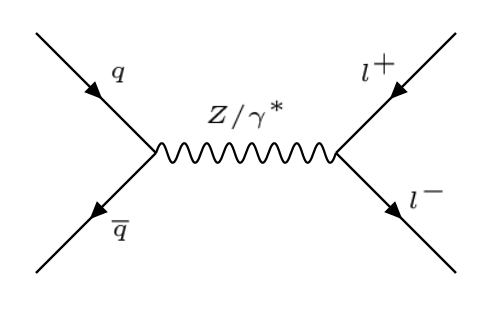
\includegraphics[scale = 0.2]{images/DY.png}
        \caption{}
        \label{fig:bckgFeynman_DY}
    \end{subfigure}
    \begin{subfigure}{.25\textwidth}
        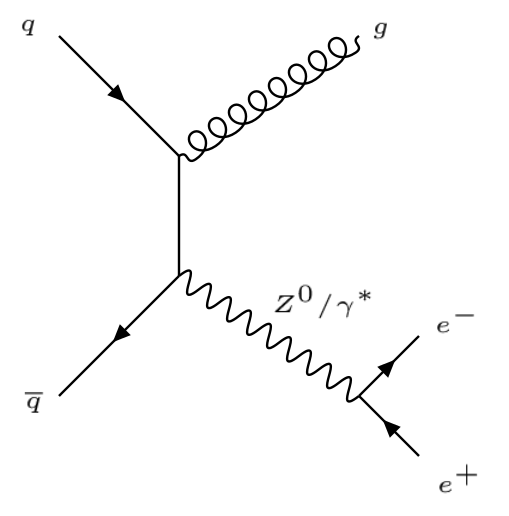
\includegraphics[height=\textwidth]{images/DY_bck.png}
        \caption{}
        \label{fig:bckgFeynman_DY_bck}
    \end{subfigure}    	
    \begin{subfigure}{.25\textwidth}
        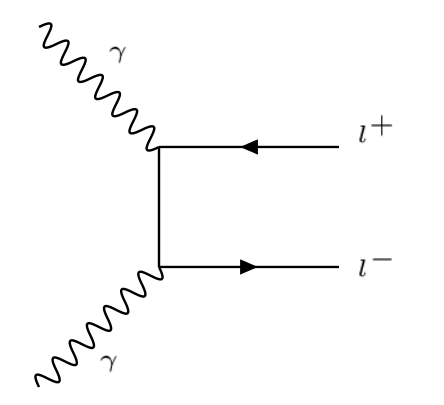
\includegraphics[scale = 0.2]{images/PI.png}
        \caption{}
        \label{fig:bckgFeynman_PI}
    \end{subfigure}	
    \begin{subfigure}{.35\textwidth}
        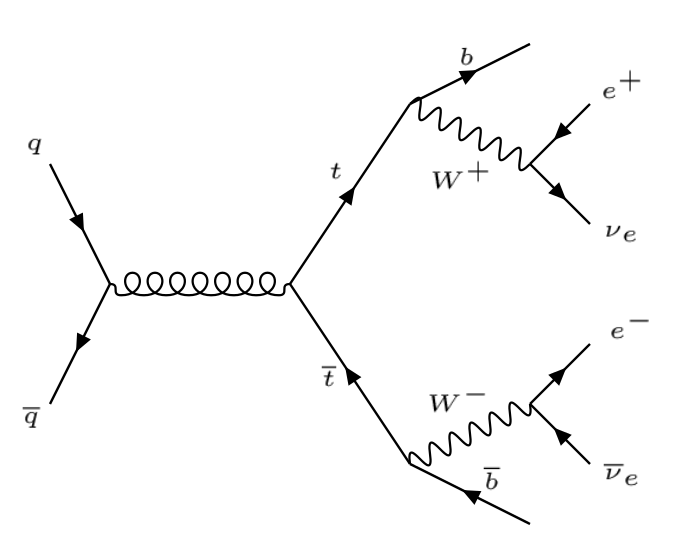
\includegraphics[height=\textwidth]{images/ttbar.png}
        \caption{}
        \label{fig:bckgFeynman_ttbar}
    \end{subfigure}
    \caption{Feynman diagrams of the leading order SM processes contributing to the background of the search for the $Z'$. The most signficant contribution comes from the Drell-Yan process, seen in (a). (b) shows the Drell-Yan process with a jet background from the emission of gluons, with (c) being the photon induced production of a dilepton pair. The top-antitop contribution is seen in (d).\label{fig:bckgFeynman2}}
\end{figure}

Feynman diagrams displaying the dominant processes contributing to the background in the experiment are shown in Figure \ref{fig:bckgFeynman}. Figures \ref{fig:bckgFeynman_DY} and \ref{fig:bckgFeynman_DY_bck} show the Drell-Yan process, in which a quark and antiquark annihilate to produce to dilepton pair through an intermediate $Z$ boson or photon. This is the main source of background events in the search for a $Z'$ boson and is to a large extent irreducible. This is due to the difficulty in distinguishing a electron positron pair produced from a Z boson compared to a potential $Z'$ boson, as the $Z'$ would have very similar properties compared to its Standard Model equivalent, save for its larger mass. The photon induced process is seen in Figures \ref{fig:bckgFeynman_PI}, and produces a dilepton pair through the interaction of two photons. Shown in Figure \ref{fig:bckgFeynman_ttbar}, the top-antitop process involves a quarks and antiquarks producing a $t\overline{t}$ pair, which undergo flavour changing through the emmission of a $W$ boson. These $W$ bosons then may produce a electron-neutrino pair.

\begin{figure}[htb]
    \centering
    \begin{subfigure}{.25\textwidth}
        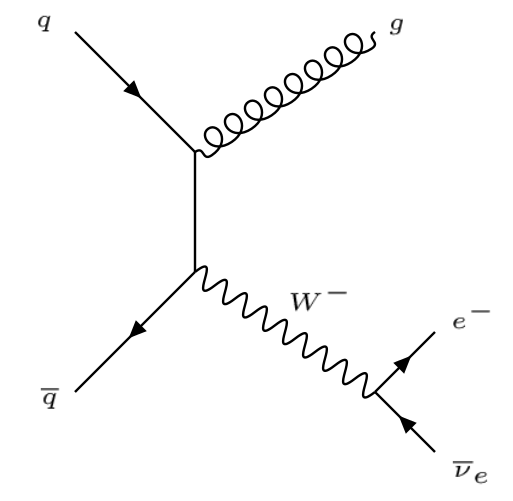
\includegraphics[height=\textwidth]{images/W_jets.png}
        \caption{}
        \label{fig:bckgFeynman_wJets}
    \end{subfigure}
    \begin{subfigure}{.25\textwidth}
        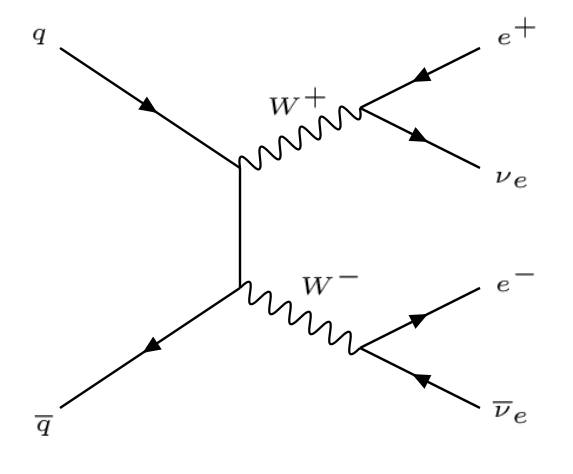
\includegraphics[height=\textwidth]{images/WW.png}
        \caption{}
        \label{fig:bckgFeynman_WW}
    \end{subfigure}
    \begin{subfigure}{.25\textwidth}
        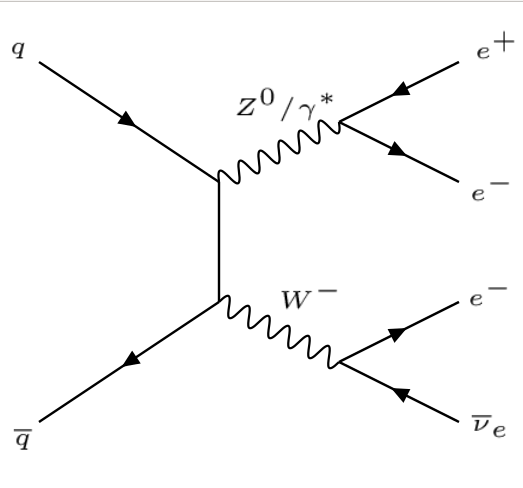
\includegraphics[height=\textwidth]{images/WZ.png}
        \caption{}
        \label{fig:bckgFeynman_WZ}
    \end{subfigure}
    \begin{subfigure}{.25\textwidth}
        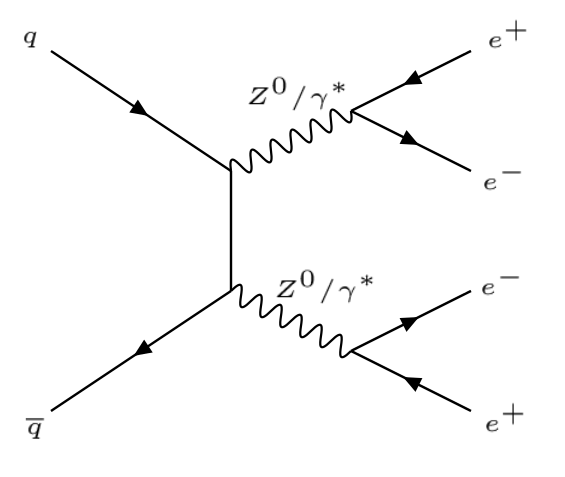
\includegraphics[height=\textwidth]{images/ZZ.png}
        \caption{}
        \label{fig:bckgFeynman_ZZ}
    \end{subfigure}
    \caption{Feynman diagrams of the leading order SM processes contributing to the background of the search for the $Z'$. The production of a $W$ boson combined with jets from the emission of a gluon is shown in (a). The diboson processes in (b), (c) and (d) are the $W^+W^-$, $WZ$ and $ZZ$ background events respectively.\label{fig:bckgFeynman}}
\end{figure}

Additional processes are shown in Figure \ref{fig:bckgFeynman}. Figure \ref{fig:bckgFeynman_wJets} shows $W+\rm{jet}$, . Figures \ref{fig:bckgFeynman_WW}, \ref{fig:bckgFeynman_WZ} and \ref{fig:bckgFeynman_ZZ} are the diboson processes $W^+W^-$, $WZ$ and $ZZ$ respectively.

\subsection{Use of Monte Carlo Simulations}%%%%%%%%

Before performing an experiment and investing a large amount of time and resources into it, it is often very useful to utilise Monte Carlo simulations in order to gain an idea of the output of an experiment. A Monte Carlo simulations utilise psuedo-random number generation to mimic probability distributions that govern the properties of a particle.

These simulations are important as they allow the user to estimate a variety of important variables in the experiment, such as the expected number of signal events under a given set of conditions, the detector resolution and the discovery significance. A set of simulated samples will be analysed in order to gather information to optimise the search for the $Z'$. 

The number of events $N$ observed in a detector during a run is given by

\begin{equation}
N = \int \mathcal{L}A\epsilon\sigma dt ,
\end{equation}
where the luminosity $\mathcal{L}$ is equivalent to the flux of particles from the accelerator passing through the interaction point and $\sigma$ is the cross section of the process that the detector is searching for. The quantity $A\epsilon$ is the quantity $\rm{acceptance} \times \rm{efficiency}$, which is defined here as the fraction of simulated candidate events that pass the event selection requirement.

By replacing the instantaneous luminosity with the integrated luminosity ${L}_{\rm{int}} = \int \mathcal{L}dt$, the number of events can be expressed as
\begin{equation}
N= \mathcal{L}_{\rm{int}}A\epsilon\sigma.
\end{equation}

The number of observed events is related to the total number of events in a binned sample through $N = A\epsilon N_{\rm{tot}}$ , therefore, a Monte Carlo sample containing $N'$ observed events at an integrated luminosity $\mathcal{L'}_{\rm{int}}$ can be scaled to the luminosity of the LHC through the expression

\begin{equation}
N = \mathcal{L}_{\rm{int}}\frac{N'}{\mathcal{L'}_{\rm{int}}} = \sigma\frac{N'}{N_{\rm{tot}}}.
\label{eqn:nEvents}
\end{equation}

Some of the samples are `binned' in to certain mass regions in order to improve the statistics of the simulated data; for example, a bin from $100\,\rm{GeV}-200\,\rm{GeV}$ would only produce simulated signal events with an invariant mass within this range. This is important as certain energy ranges may have a much lower cross section than others, meaning an unbinned sample set would have to be much larger to reduce the statistical uncertainties in less probable regions. The effect of having bins with different cross sections but the same number of events corresponds to a change in the effective luminosity used to generate the sample set. After analysing each bin, they are scaled using Equation (\ref{eqn:nEvents}) and then `stitched' back together.

The Monte Carlo samples in this paper have all been scaled to an integrated luminosity of $20.3\,\rm{fb}^{-1}$, which was the integrated luminosity of the LHC during the 2012 run.

In total, four different sample sets were used in this paper. These were a Drell-Yan sample, binned into 14 subsets that ranged up to $3\,$TeV, a $Z'$ at $1.5$, $2$ and $2.5$ TeV, an unbinned diboson sample containing $WW$, $WZ$ and $ZZ$ events, and an unbinnned $t\overline{t}$ sample.

\begin{figure}[h]
    \centering
    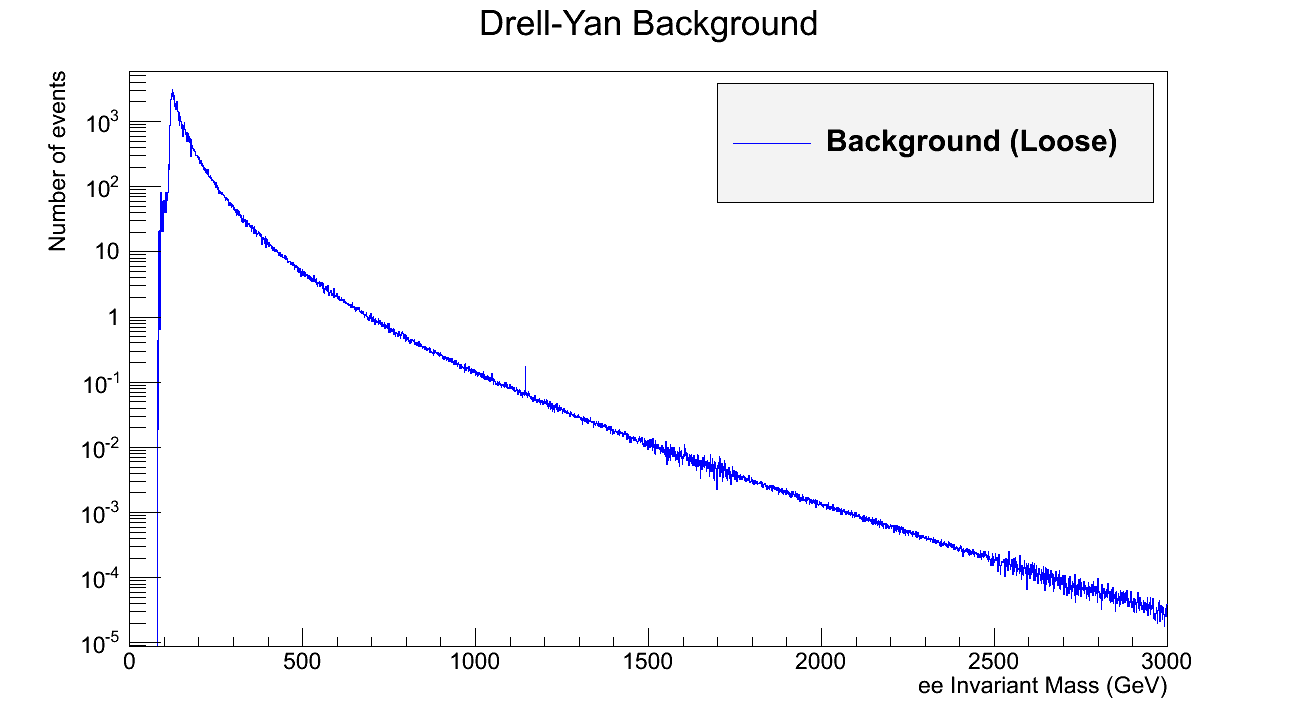
\includegraphics[scale=0.01]{images/DYBackground.png}
    \caption{The simulated background from Drell-Yan events using a loose selection criteria.}
\end{figure}

\section{Cuts and Event Selection}
\label{sec:cuts}
A \textit{cut} is a selection applied to a set of data in order to remove some of the background while retaining as many signal events as possible to improve the purity of the collected data. In the case of a linear cut, this may be accepting or rejecting events that have an energy above a certain value. This concept can be extended to \textit{multivariate cuts}, where a linear combination of variables $x_i$ form a selection $t$ of the form

\begin{equation}
t = \sum_{i=1}^{n}\alpha_i x_i < t_{cut}.
\end{equation}

Here, the optimum values of the coefficients $\alpha_i$ would have to be determined using some multivariate analysis technique.

\subsection{ATLAS Electron Selection Criteria}
\label{sec:cuts_selection}
Loose, medium and tight refer to an increasingly stringent set of selection criteria for 'good' electrons that apply a set of cuts that are introduced in \cite{expectedElectronPerformance}.

The true source of electron candidates can usually classified into one of four discrete categories. 
Isolated electrons are signatures that match a `true' electron (ie the particle that caused a signature to be detected was in fact an electron species) originating from a $W$ or $Z$ boson, for example. Conversely, hadron fakes are those that do not match a true electron, muon or tau, and are caused by jets faking the signature of an electron.
Non-isolated electrons are true electrons originating from a meson decay, while background electrons are those produced from photon pair production, such as when photons are produced in brehmsstrahlung or Dalitz decays.

The jet rejection for loose, medium and tight is around 500, 5000 and $5\times10^4$  respectively \cite{ElectronPerformanceMeasurements}. The electron is reconstructed by associating an energy signature and track. The EM calorimeter identifies the energy via a clustering algorithm and associates it to a track. 

The variables defining the loose, medium and tight criteria are shown in Tables \ref{table:looseVariables}, \ref{table:mediumVariables} and \ref{table:tightVariables}.

\begin{table}[h!t]
\caption{ Variables Associated with the loose selection criteria \cite{ElectronPerformanceMeasurements}\label{table:looseVariables}}
\begin{tabular}{|p{5cm}|p{8cm}|p{1cm}| } 
\hline
\multicolumn{3}{|c|}{\textbf{Loose}}		\\\hline
Type&Description&Name		    \\\hline
Acceptance &  $|\eta|<2.47$ &  	\\\hline
\multirow{2}{*}{Hadronic Leakage} & Ratio of transverse energy $E_{\rm{T}}$ in the first layer hadronic calorimeter to $E_T$ of the EM cluster. Used in the ranges $|\eta|<0.8$ and $|\eta|<1.37$ & $R_{\rm{had,1}}$ \\\cline{2-3}
& Ratio of $E_T$ in hadronic calorimeter to $E_T$ of the EM cluster. Used in the range $0.8<|\eta|<1.37$ & $R_{\rm{had}}$\\\hline
\multirow{2}{*}{Middle Layer of EM calorimeter} & Ratio of the energy in $3\times7$ cells ($E237$) over the energy in $7\times7$ cells ($E277$) centred at the electron cluster position & $R_{\eta}$ \\\cline{2-3}
& Lateral shower width, $ \sqrt{\frac{\sum E_i \eta_{i}^{2}}{\sum E_i} - \left( \frac{\sum\eta_i}{\sum E_i} \right)^2 }$ calculated over a window of $3\times5$ cells & $\omega_{\eta^2}$ \\\hline
\end{tabular}
\end{table}

\begin{table}[h!t]
\centering
\caption{ Variables Associated with the medium selection criteria \cite{ElectronPerformanceMeasurements}\label{table:mediumVariables}}
\begin{tabular}{|p{5cm}|p{8cm}|p{1cm}| } 
\hline
\multicolumn{3}{|c|}{\textbf{Medium (includes loose with tighter requirements on shower shapes)}} \\\hline
Type&Description&Name		    \\\hline
\multirow{2}{*}{Strip layer of EM calorimeter} & Shower width, $\sqrt{ \frac{\sum E_i (i-i_{\rm{max}})^2 } {\sum E_i} }$, summed over the strups in a window of dimesions of $\Delta\eta\times\Delta\phi\approx 0.0625\times0.2$, corresponding typically to 20 strips in $\eta$, and $i_{\rm{max}}$ is the index of the highest-energy strip. & $\omega_{\rm{stot}}$ \\\cline{2-3}
& The energy deposition ratio $\frac{E_1/E_2}{E_1+E_2}$ where $E_1$ and $E_2$ are the largest and second largest energy depositions in the cluster. & $E_{\rm{ratio}}$ \\\hline
\multirow{3}{*}{Track Quality} & Number of hits in the pixel detector ($\geq$1)&$n_{\rm{pixel}}$ \\\cline{2-3}
& Number of total hits in the pixel and SCT detectors ($\geq$7) & $n_{\rm{Si}}$ \\\cline{2-3}
& Transverse impact parameter ($|d_0|<5\,$mm) & $d_0$ \\\hline
Track-cluster matching & $\Delta\eta$ between the cluster position in the strip layer and the extrapolated track ($|\Delta\eta|<0.01$) & $\Delta\eta$\\\hline
\end{tabular}
\end{table}

%\begin{table}[h!t]
%\centering
%\caption{ Variables Associated with the tight selection criteria%\cite{ElectronPerformanceMeasurements} \label{table:tightVariables}}
%\begin{tabular}{|p{5cm}|p{8cm}|p{1cm}| } 
%\hline
%\multicolumn{3}{|c|}{\textbf{Tight (includes medium)}}\\\hline
%Type&Description&Name		    \\\hline
%\multirow{3}{*}{Track-cluster matching} & $\Delta\phi$ between the cluster position in the middle layer and the extrapolated track ($|\Delta\phi|<0.02$) & $\Delta\phi$ \\\cline{2-3}
%&Ratio of cluster energy to track momentum &$E/p$\\\cline{2-3}
%& Tighter $\Delta\eta$ requirement ($\Delta\eta<0.005$) & $\Delta\eta$\\\hline
%Track quality & Tighter transverse impact parameter ($|d_0|<1\,$mm) & $d_0$\\\hline
%\multirow{2}{*}{TRT} & Total number of hits in the TRT & $n_{\rm{TRT}}$\\\cline{2-3}
%& Ratio of the number of high threshold hits to the total number of hits in the TRT & $f_{\rm{HT}}$\\\hline
%\multirow{2}{*}{Conversions} & number of hits in the b-layer ($\geq$1) & $n_{\rm{BL}}$\\%\cline{2-3}
%& Veto electron candidates matched to reconstructed photon conversions & \\\hline
%\end{tabular}
%\end{table}

\subsection{Event Selection}

For an event that passes the chosen trigger, there are a number of electrons may not be associated with the signal. Therefore, it is important to identify the dilepton pair associated with the $Z'$ decay if it is indeed present in the event. 

Firstly, a fiducial volume is defined by applying the cut $|\eta|<2.47$ to ensure that background radiation from the detector or external radiation is not included. Therefore electrons outside of this fiducial volume is rejected. 
The electrons located in the crack between the barrel and endcap $1.37\leq|\eta|\leq1.52$.
The transverse energy of the electron $E_T$ is required to be greater than than $30\,$GeV. 
The electron is required to pass the required electron selection criteria, which initially will be the loose criteria.
The two electrons with the highest $P_T$ sum are chosen, and the invariant mass of the pair is rejected if it is lower than $80\,$GeV.

%For the highest $P_T$ and next highest $P_T$ electron, known as the leading and subleading electrons, a calorimeter cluster isolation requirement is applied, corresponding to two linear expressions

%\begin{equation}
%\begin{split}
%\rm{leading\,\,isolation} & <0.007P_T + 5.0\,\rm{GeV}\\
%\rm{subleading\,\,isolation} & <0.0022P_T + 6.0\,\rm{GeV}\\
%\end{split}
%\end{equation}

%where the isolation for the candidate electron is stored in the variable $E_T\rm{cone}20$. This cut is applied to reduce the jet background.

\begin{figure}[h]
    \centering
    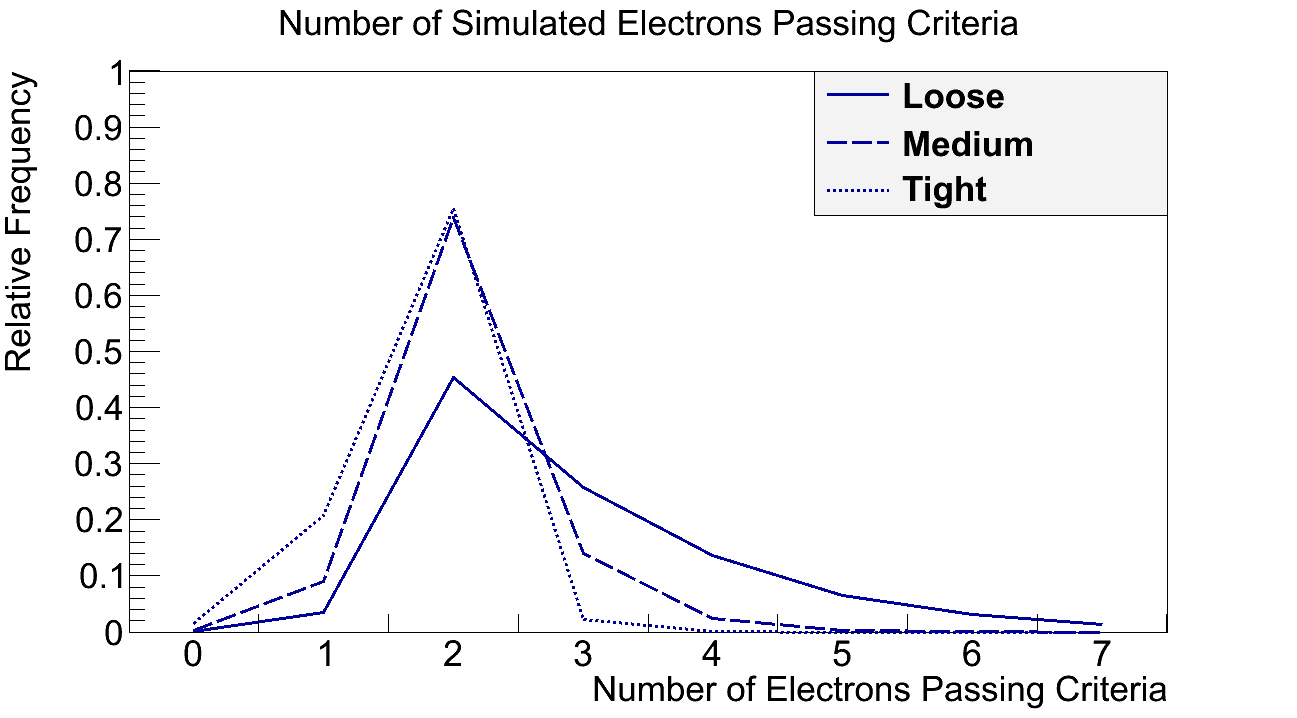
\includegraphics[scale=0.3]{images/nEl.png}
    \caption{The number of simulated electrons passing each selection criteria in a given event. It can be seen that a significant number of simulated events contain more than 2 electrons passing the loose and medium selection criteria. \label{fig:nEl}}
\end{figure}

An additional requirement that may also be applied is that the two final state electrons must be of an opposite sign. Theoretically, this is required in order to ensure charge conservation, though the charge of a lepton may be incorrectly identified by the detector, potentially causing genuine signal events to be discarded. However, from Figure \ref{fig:nEl} it can be seen that a substantial amount of simulated events contain more than two electrons passing the loose and medium selection criteria. Therefore, in order to reduce the possibility of a background electron being misidentified as part of the dilepton final state, the charge requirement will be  invoked during the event selection process. The efficiencies when broken down by criteria can be seen in Table \ref{table:selectionEfficiency}, and as a function of invariant mass in Figure \ref{fig:acceptance}. It can be seen that the acceptance rates for Drell-Yan and $Z'$ events in Figure \ref{fig:acceptance} and very close; this is consistent with what is expected, as the 

\begin{table}[h!t]
\caption{The efficiency of the event selection process is broken down for various simulated samples. For each criteria, the percentage of initial events remaining once the selection criteria has been applied is shown, then after applying the constraints on invariant mass and opposite charge requirements. \label{table:selectionEfficiency}}
\begin{tabular}{|c|c|c|c|c|c|c| } 
\hline
Criteria & $1.5\,\rm{TeV}\,\,Z'$ & $2.0\,\rm{TeV}\,\,Z'$ & $2.5\,\rm{TeV}\,\,Z'$ & Drell-Yan & Diboson & $t\overline{t}$ \\
\hline
\bf{Loose} & $(79.4\pm0.4)\%$ & $(80.5\pm0.4)\%$ & $(81.0\pm0.5)\%$ & $(73.2\pm0.1)\%$ & $(5.41\pm0.03)\%$ & \\
Inv Mass & $(78.5\pm0.4)\%$ & $(79.7\pm0.4)\%$ & $(80.1\pm0.4)\%$ & $(72.1\pm0.1)\%$ & $(4.34\pm0.02)\%$ & \\
Opp. Charge & $(72.9\pm0.4)\%$ & $(72.6\pm0.4)\%$ & $(72.2\pm0.4)\%$ & $(66.9\pm0.1)\%$ & $(4.11\pm0.03)\%$ & \\
\hline
\bf{Medium} & $(75.6\pm0.4)\%$ & $(76.4\pm0.4)\%$ & $(77.1\pm0.4)\%$ & $(69.6\pm0.1)\%$ & $(4.49\pm0.03)\%$ & \\
Inv Mass & $(75.3\pm0.4)\%$ & $(76.1\pm0.4)\%$ & $(76.8\pm0.4)\%$ & $(69.2\pm0.1)\%$ & $(4.06\pm0.03)\%$ & \\
Opp. Charge & $(69.8\pm0.4)\%$ & $(69.1\pm0.4)\%$ & $(69.1\pm0.4)\%$ & $(64.0\pm0.1)\%$ & $(3.94\pm0.03)\%$ & \\
\hline
\bf{Tight} & $(65.8\pm0.4)\%$ & $(66.8\pm0.4)\%$ & $(67.2\pm0.4)\%$ & $(59.8\pm0.1)\%$ & $(3.3\pm0.02)\%$ & \\
Inv Mass & $(65.7\pm0.4)\%$ & $(66.8\pm0.4)\%$ & $(67.1\pm0.4)\%$ & $(59.8\pm0.1)\%$ & $(3.14\pm0.02)\%$ & \\
Opp. Charge & $(61.3\pm0.4)\%$ & $(61.0\pm0.4)\%$ & $(60.8\pm0.4)\%$ & $(55.7\pm0.1)\%$ & $(3.07\pm0.02)\%$ & \\
\hline
\end{tabular}
\end{table}

\begin{figure}[htb]
	\centering
    \begin{subfigure}{.49\textwidth}
    	\raggedleft
        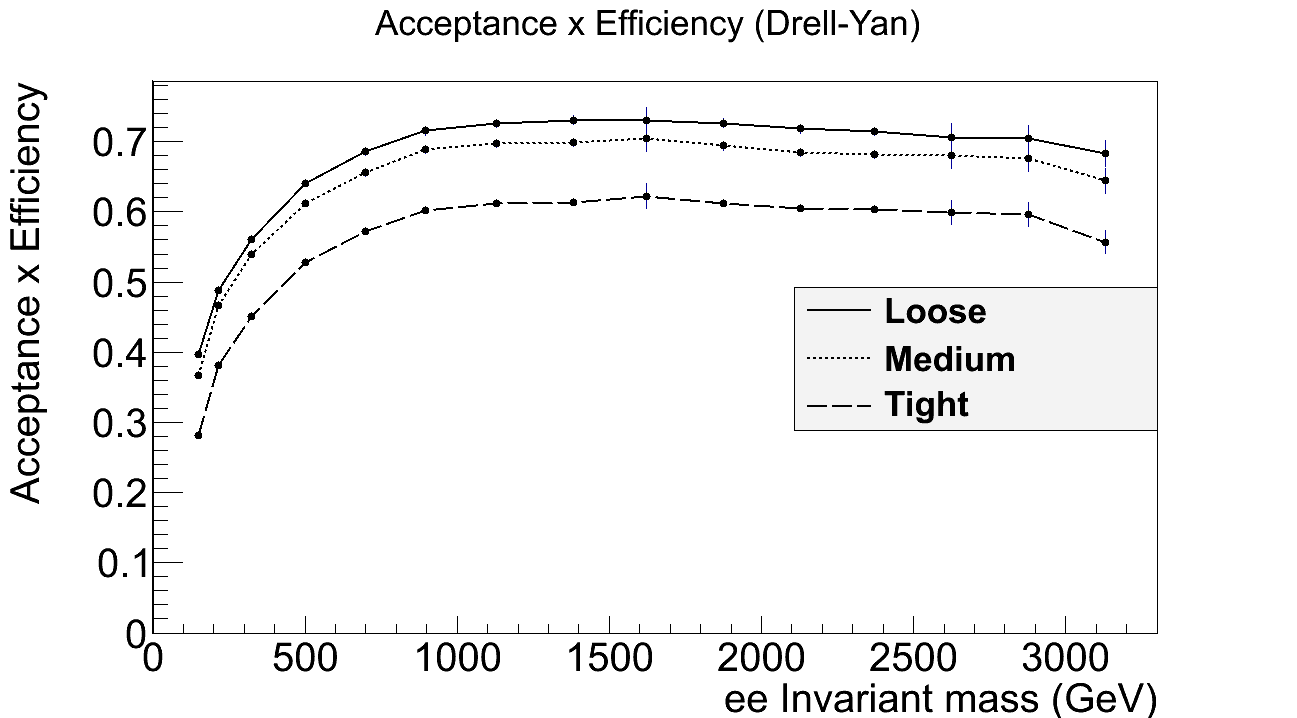
\includegraphics[width=1.13\textwidth]{images/acceptanceDY.png}
        \caption{}
        \label{fig:acceptanceDY}
    \end{subfigure}
    \begin{subfigure}{.49\textwidth}
    	\raggedright
        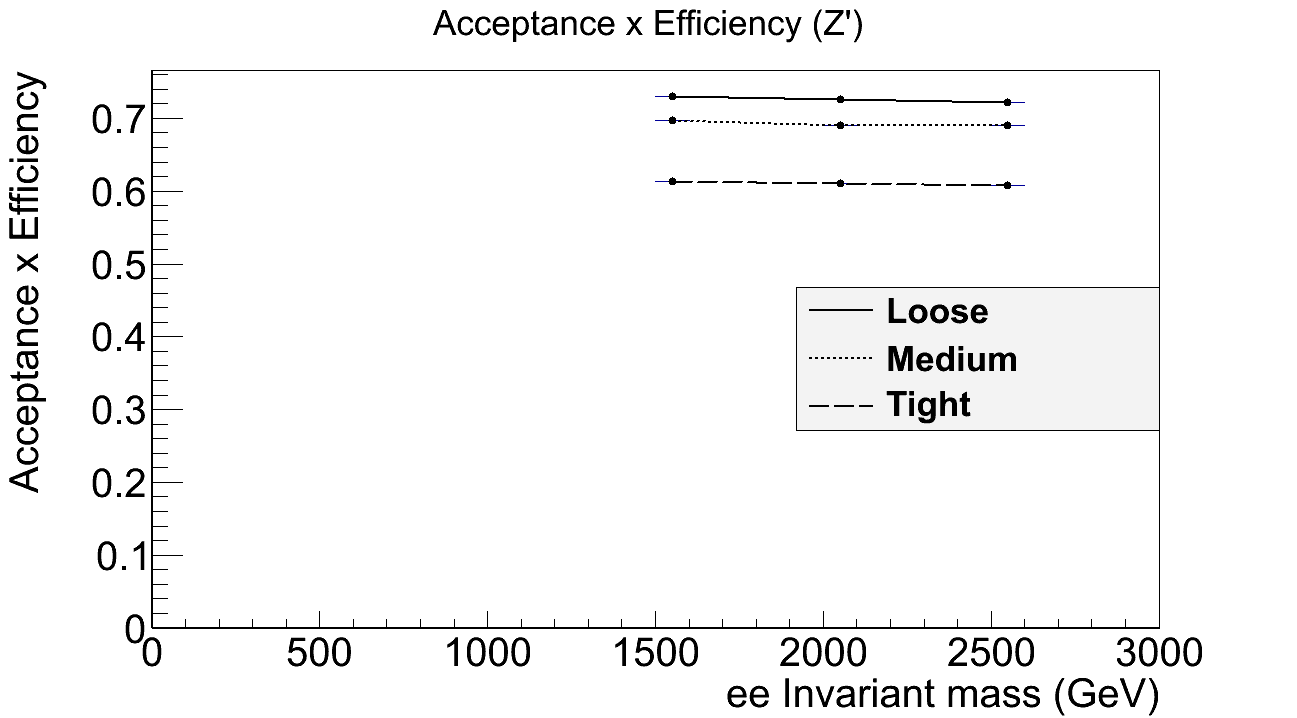
\includegraphics[width=1.13\textwidth]{images/acceptanceZ.png}
        \caption{}
        \label{fig:acceptanceZ}
    \end{subfigure}    	
    \caption{ The $\rm{acceptance}\times\rm{efficiency}$ is plotted as a function of energy for the Drell-Yan and $Z'$ samples. It can be seen that the fractional number of events that are identified are approximately equal. \label{fig:acceptance}}
\end{figure}



\section{Monte Carlo Simulated Analysis}
\label{sec:MonteCarloSimulatedAnalysis}

\subsection{$Z'$ Simulated Events}
 
As there is a range of masses at which the $Z'$ could appear, it is important to study samples at various masses in order to determine the most appropriate search conditions for the experiment. Three different $Z'$ sample sets were used in this paper, at masses of $1500\,$GeV, $2000\,$GeV and $2500\,$GeV. While these masses have been ruled out by previous searches, it is still useful to use these samples as the information provided is stil relevant to searches at higher masses. 

A resonant peak occurs in an experiment as the cross section for the production of a particle, in this case a $Z'$ boson, increases in a certain energy range. The width of the resonance peak is related to the lifetime of the $Z'$ through the equation 

\begin{equation}
\Gamma = \frac{\hbar}{\tau},
\end{equation}

where $\Gamma$ is the Full Width at Half Max (FWHM) of the peak. The width is also convoluted from the minimum resolution of the detector.
Using the minimisation library Minuit \cite{Minuit}, the $Z'$ peaks are fitted to a Breit-Wigner distribution of the form

\begin{equation}
B(E;M,\Gamma) = \frac{k}{(E^2 - M^2)^2 + M^2\Gamma^2},
\end{equation}

where 

\begin{equation}
k = \frac{2\sqrt{2}M\Gamma\gamma}{\pi\sqrt{M^2 + \gamma}}, \,\, \gamma = \sqrt{M^2(M^2 + \Gamma^2)}.
\end{equation}

The output of this fitting process can be seen in Figure \ref{fig:ZPrimePeaks}.

\begin{figure}[htb]
	%\centering
    \begin{subfigure}{.5\textwidth}
        \raggedleft
        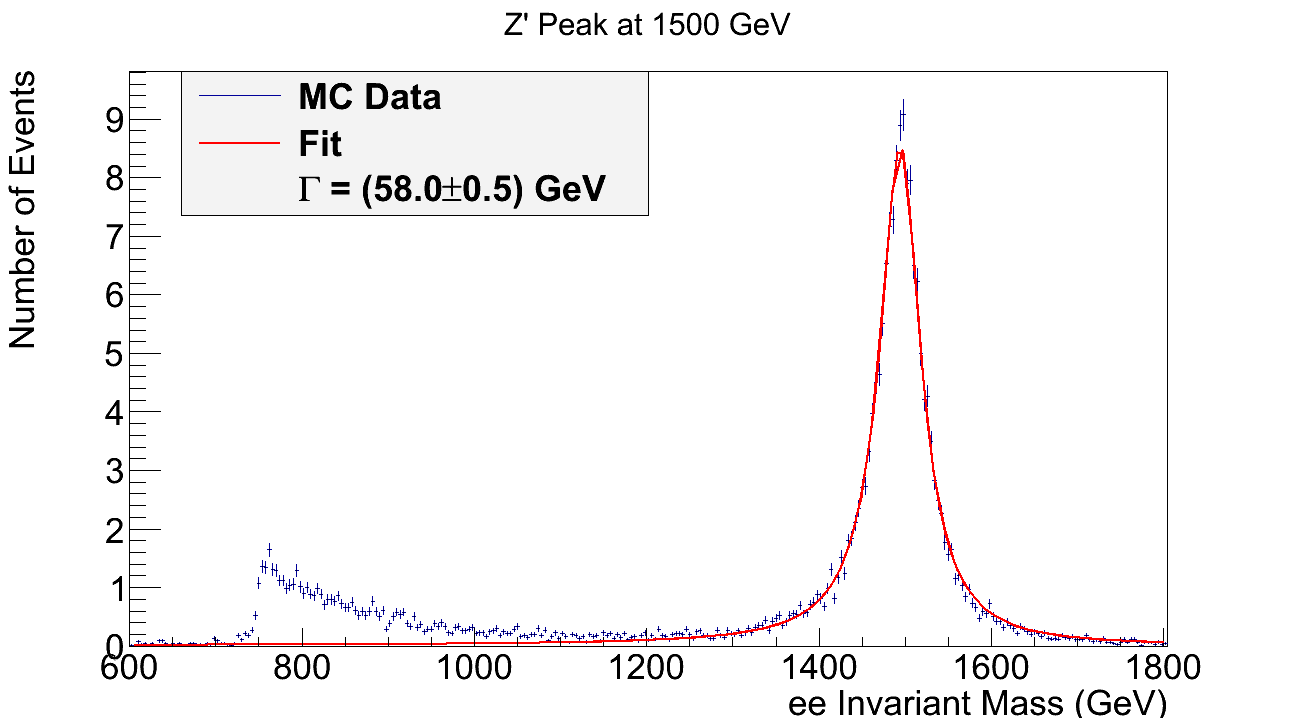
\includegraphics[width=\textwidth]{images/Z1500.png}
        \caption{}
        \label{fig:Z1500}
    \end{subfigure}
    \begin{subfigure}{.5\textwidth}
       	\raggedright
        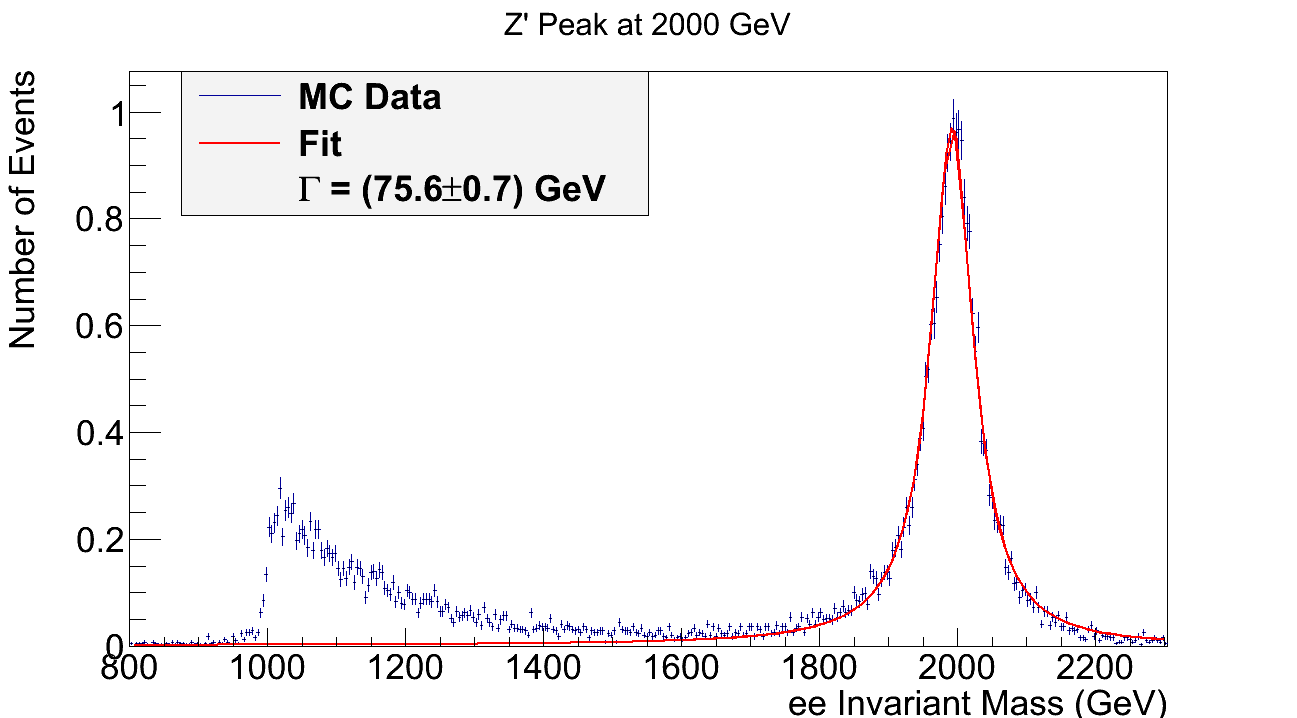
\includegraphics[width=\textwidth]{images/Z2000.png}
        \caption{}
        \label{fig:Z2000}
    \end{subfigure}	
    \begin{subfigure}{.5\textwidth}
    	\centering
        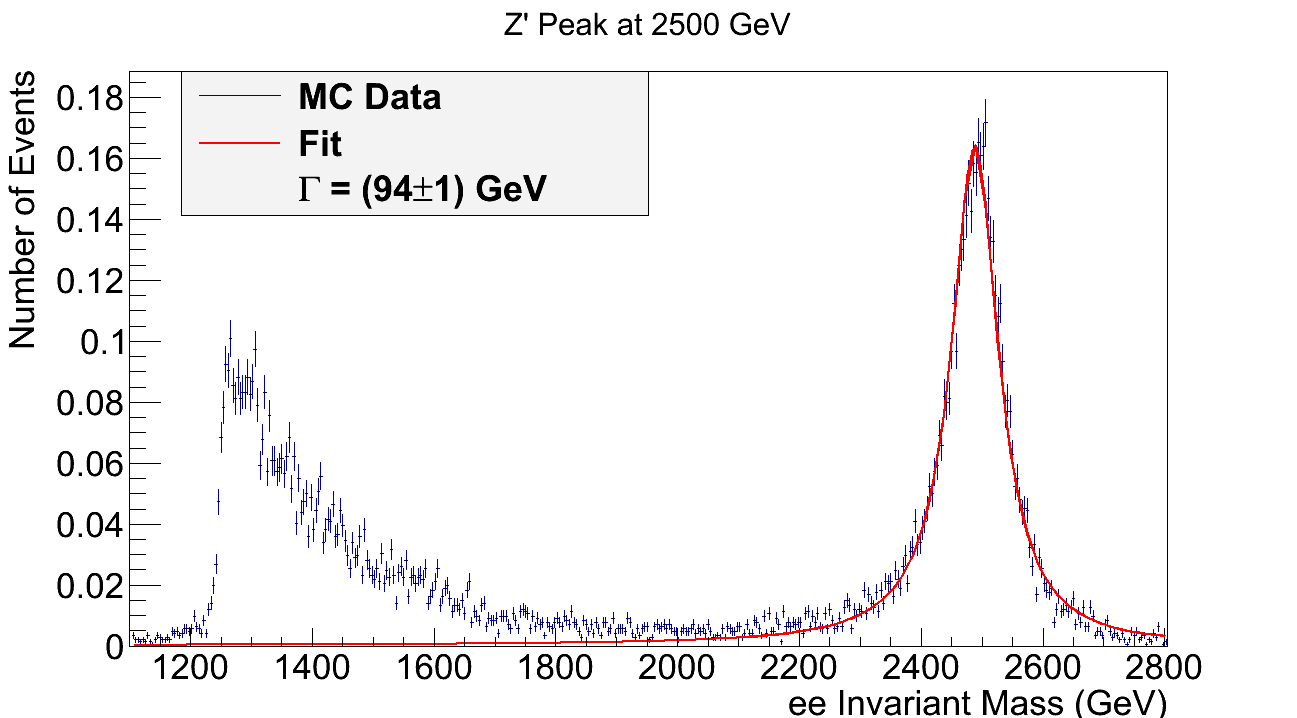
\includegraphics[width=\textwidth]{images/Z2500.png}
        \caption{}
        \label{fig:Z2500}
    \end{subfigure}
    \caption{The SSM $Z'$ resonance peak is fitted to a relativistic Breit-Wigner distribution at masses of (a) $1500\,$GeV (b), $2000\,$GeV and (c) $2500\,$GeV. \label{fig:ZPrimePeaks}}
\end{figure}

As well as the resonance peak, a second peak caused by energy loss from bremsstrahlung processes can be seen. 

The retrieved value for $\Gamma$ computed during the minimisation process for the different masses is tabulated in Table \ref{table:resonanceWidth}, as well as the number of events observed from the simulated data $N_{\rm{tot}}$ and the expectation value for this sample at the given luminosity.

\begin{table}[h!t]
\centering
\caption{The FWHM $\Gamma$ is calculated by fitting each $Z'$ peak to a relativistic Breit-Wigner distribution using Minuit. The total number of events from the  MC sample at $20.3\,\rm{fb}^{-1}$, $N_{\rm{tot}}$, and the expected number of events $E[N]$, are also shown. \label{table:resonanceWidth}}
\begin{tabular}{ |c|c|c|c|c| } 
\hline
$Z'$ mass (GeV) & $\Gamma\,$(GeV) & $\frac{\Gamma}{M_{Z'}}$ & $N_{\rm{tot}}$ & $E[N]$\\
\hline
1500 & $58.0\pm0.5$ & $0.0387\pm0.0003$ & $240\pm1$			& $240\pm20$\\
2000 & $75.6\pm0.7$ & $0.0378\pm0.0004$ & $41.0\pm0.2$		& $41\pm6$\\
2500 & $94\pm1$ & $0.0376\pm0.0004$ 	& $11.19\pm0.06$	& $11\pm3$\\
\hline
\end{tabular}
\end{table}

From the table, it can be calculated that the average width of the $Z'$ peak as a fraction its mass is $\frac{\Gamma}{M_{Z'}} = 0.0380\pm0.0002$.

\begin{figure}[h]
    \centering
    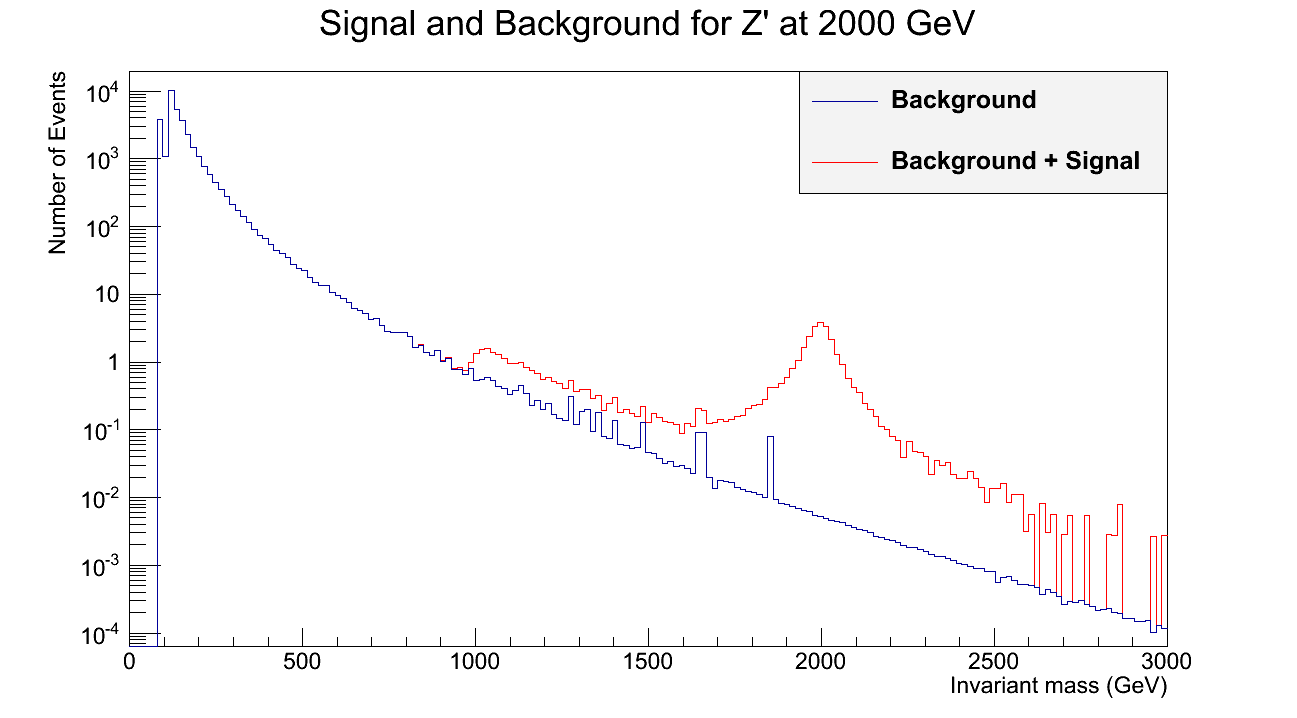
\includegraphics[scale=0.3]{images/backgroundSignal.png}
    \caption{ The background and signal spectra for a $Z'$ at $2000\,$TeV. \label{fig:backgroundSignal}}
\end{figure}


\subsection{Discovery Significance}

In order to claim a discovery, a signal must be detected to a significance of $5\sigma$. Therefore, it is important to modify the search such that the maximum significance can be achieved for a given number of signal events. In this section, the Monte-Carlo data will be analysed to determine the optimum method of discovery.

There are a number of different means of analysis that can be undertaken to search for the existance of a new particle. Firstly, the obtained data could be fitted to a template representing the expected distribution of events for a particle predicted by a given model. However, this is a model dependant means of searching for new particles. A more model independant approach is by looking at the number of events $n$ within a window covering a certain energy range, and comparing the number of events observed to the expected background. Another approach is to count the number of events that occur above a critical energy. These two approaches will be compared in this section.

As described in \cite{Cowan:2010js}, the median discovery significance $Z_0$ for an experiment with a known background can be expressed as

\begin{equation}
Z_0 = \begin{cases}
    \sqrt{2\left(n\log\frac{n}{b}+b-n \right)} & \widehat{\mu}\geq0\\        0         & \widehat{\mu}\leq0,
\end{cases}
\end{equation}

where the estimator $\widehat{\mu}=n-b$. Under the condition $\widehat{\mu}\geq0$ and using the number of events $n=s+b$ the discovery significance can be expressed as 

\begin{equation}
Z_0 = \sqrt{2\left(  (s+b)\ln\left(1+\frac{s}{b}\right)  - s \right)}.
\label{eqn:asimov}
\end{equation}

The discovery significance can be approximated as $Z_0\approx s/\sqrt{b}$ which is valid for $s<<b$; however given the low background compared to the number of events in models in which have a high cross section for the $Z'$, such as the SSM, the expression is not valid and so the full form is used.

Using Equation \ref{eqn:asimov}, the median discovery significance is calculated for a search window centered on the $Z'$ resonance peak as a function of the width of the window. The discovery significance is also calculated for using the second method, and is plotted as a function of the critical energy.

\begin{figure}[htb]
    \centering
    \begin{subfigure}{.49\textwidth}
        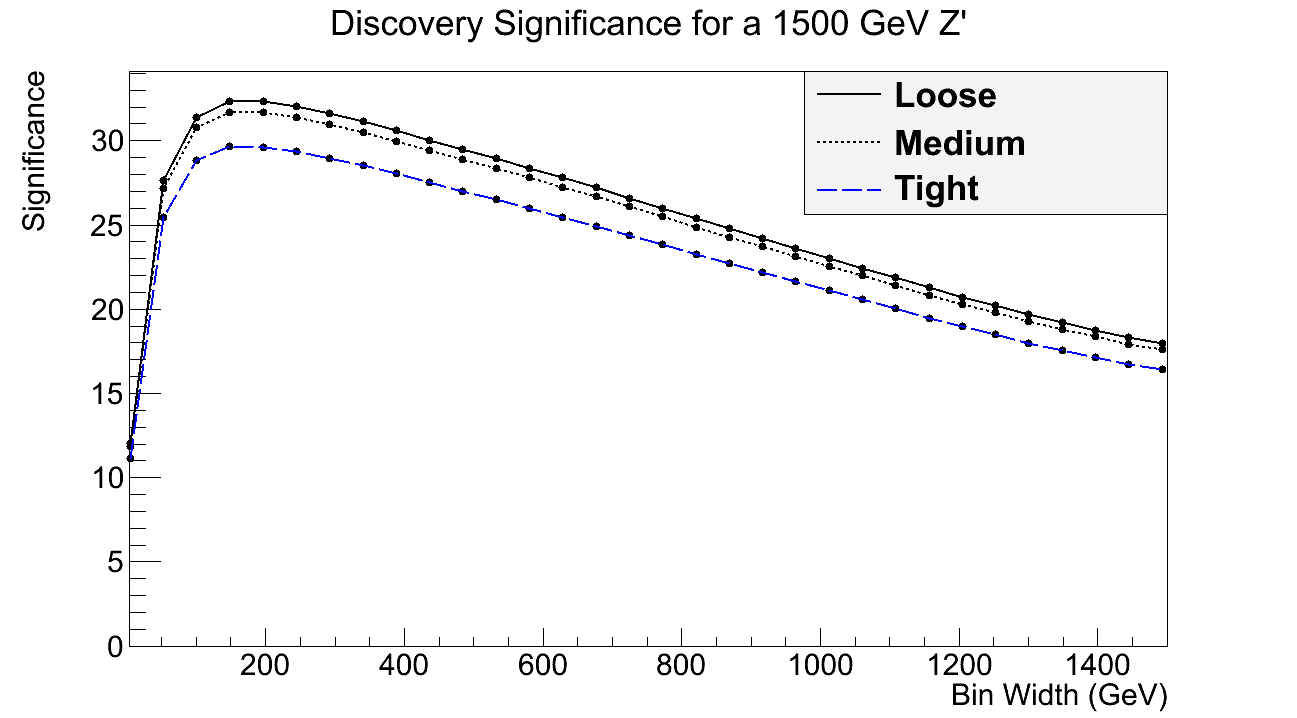
\includegraphics[height=0.6\textwidth]{images/DS1500.png}
        \caption{}
        \label{fig:DS1500}
    \end{subfigure}	
    \begin{subfigure}{.49\textwidth}
        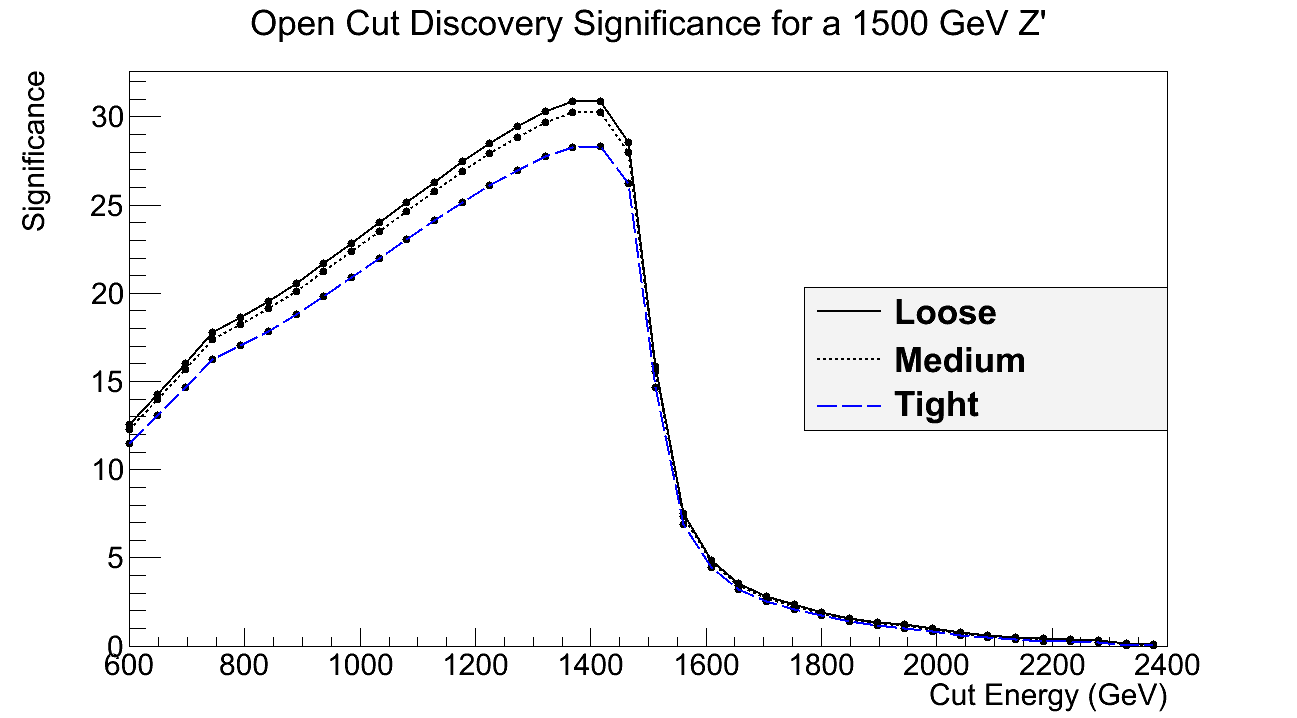
\includegraphics[height=0.6\textwidth]{images/IDS1500.png}
        \caption{}
        \label{fig:IDS1500}
    \end{subfigure}
    \caption{ (a) The discovery significance of a $1500\,$GeV $Z'$ is plotted as a function of the width of the search region, centered around the $Z'$ peak. It can be seen that the discovery significance plateus at around $120\,$GeV. (b) The discovery significance of the $1500\,$GeV $Z'$ is calculated, using the entire region above a given energy to search in. It can be seen that the overall significance is slightly less than using a search window. \label{fig:DiscoverySignificance}}
\end{figure}

These two methods can be seen in Figure \ref{fig:DiscoverySignificance}. In \ref{fig:DS1500}, it can be seen that the discovery significance reaches a maximum at a window width of around $170\,$GeV. The optimum width appears to be independant of the selection criteria used; this is consistent with what is expected as the Drell-Yan background is irreducible, and the $\rm{acceptance}\times\rm{efficiency}$ as a function of invariant mass follows the same general form for both Drell-Yan and $Z'$ leptons. Therefore, applying a stricter criteria will simply scale the DY background  and signal values by a certain factor. 


In Figure \ref{fig:IDS1500}, the discovery significance for the open cut method is plotted as a function of the critical energy. It can be seen that the maximum discovery significance obtained using this method is only slightly lower than using a search window. This is somewhat un-intuitive as one would naturally expect the number of additional background events obtained at energies above the $Z'$ peak to substantially reduce the discovery significance obtained. However, given that the Drell-Yan background becomes increasingly small at higher energies and the fairly high cross section of the SSM $Z'$, this suppresses the impact of the additional background events decreasing the significance.

\begin{table}[h!t]
\label{table:discoverySignificance}
\centering
\caption{The discovery significances for the two methods described in this section are listed. Left to right: the mass of the $Z'$ sample used in this calculations; the electron ID criteria used; the bin width that generates the largest discovery significance, $Z_0$, using a search window; the discovery significance obtained with a search window at this width; the open cut value that provides the largest value; the significance obtained using this open cut. It can be seen that using a search window provides a slightly greater discovery significance than the open cut method.}
\begin{tabular}{ |c|c|c|c|c|c| } 
\hline
$Z'$ mass (GeV) &  ID Criteria & Best Search Width (GeV) & Maximum $Z_0$ & Best Open Cut (GeV) &Maximum $Z_0$\\
\hline
\multirow{3}{*}{$1500$}  & Loose & \multirow{3}{*}{$160\pm4$}& $32.4\pm0.2$ & \multirow{3}{*}{$1392\pm4$} &$31.0\pm0.1$ \\\cline{2-2}\cline{4-4}\cline{6-6}
& Medium  & & $31.7\pm0.2$ & & $30.4\pm0.1$\\\cline{2-2}\cline{4-4}\cline{6-6}
& Tight &  & $29.7\pm0.2$ & & $28.4\pm0.1$\\\hline
\multirow{3}{*}{$2000$} & Loose & \multirow{3}{*}{$256\pm4$}& $12.38\pm0.06$ & \multirow{3}{*}{$1872\pm4$} & $12.00\pm0.06$\\\cline{2-2}\cline{4-4}\cline{6-6}
&  Medium & & $12.10\pm0.06$ & & $11.74\pm0.06$ \\\cline{2-2}\cline{4-4}\cline{6-6}
&  Tight & & $11.35\pm0.06$ & & $11.01\pm0.06$\\\hline
\multirow{3}{*}{$2500$} &  Loose & \multirow{3}{*}{$292\pm4$}& $5.86\pm0.03$ & \multirow{3}{*}{$2340\pm4$} & $5.75\pm0.03$ \\\cline{2-2}\cline{4-4}\cline{6-6}
&  Medium & & $5.74\pm0.03$ & & $5.63\pm0.03$\\\cline{2-2}\cline{4-4}\cline{6-6}
&  Tight  & & $5.37\pm0.03$ & & $5.28\pm0.03$\\\hline
\end{tabular}
\end{table}

\subsection{Variables and Linear Cuts}

In this section, lepton variables are investigated and possible linear cuts are introduced in order to cut out background events while maintaing as much of the signal as possible. The variables plotted are the background spectrum for Drell-Yan, $t\overline{t}$ and diboson events as well as a $Z'$ at $1.5\,$TeV.

\subsubsection{Transverse Energy}

The transverse energy $E_T$ is the component of energy perpendicular to the beam line and is defined as 

\begin{equation}
E_{T} = \sqrt{m^2 + P_{T}^2},
\end{equation}

where $m$ is the mass of the particle and $P_T$ is the transverse momenta. Given that the two beams of protons are colliding head on, the longtitudinal compontent of momentum is neglibigle. However, the individual partons inside the protons colliding together may themselves have some transverse component. High $P_T$ events often indicate interesting physical processes.

\begin{figure}[h]
    \centering
    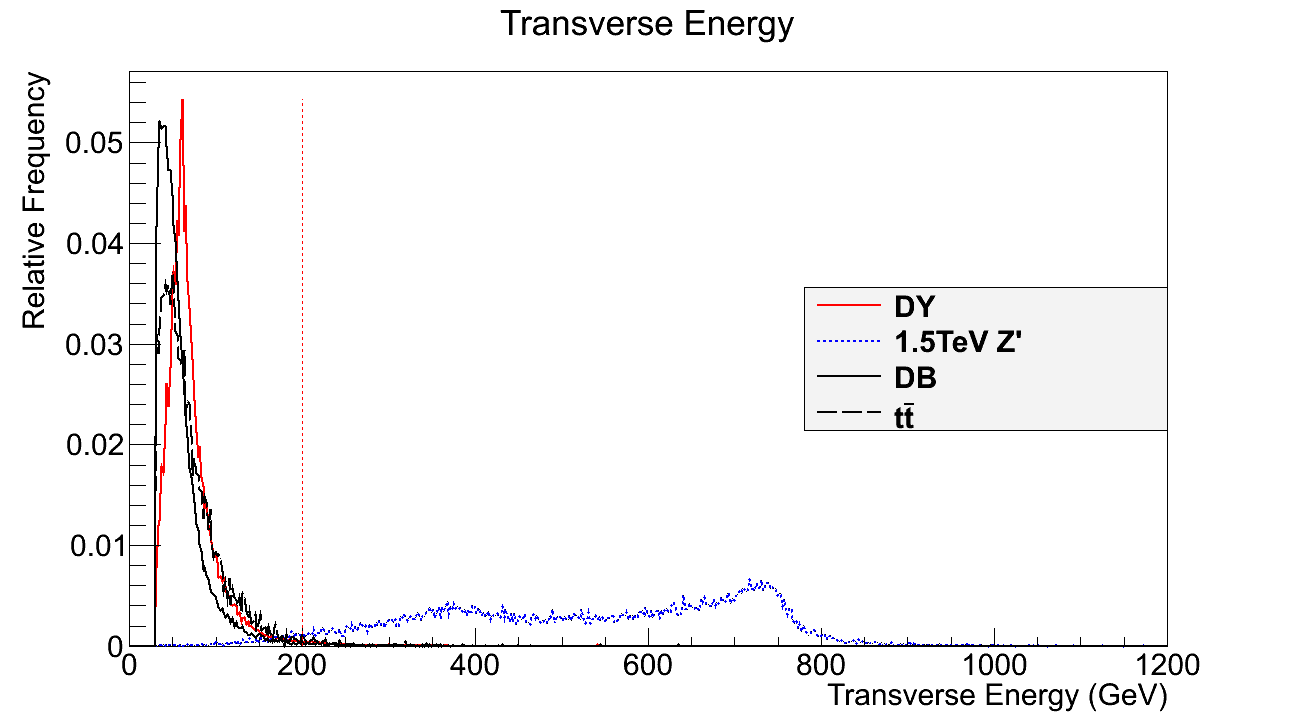
\includegraphics[scale=0.25]{images/variables/Et.png}
    \caption{The transverse energy is plotted for various samples. The dashed line shows the minimum cut on $E_T$, which is placed at $200\,$GeV. \label{fig:Et} }
\end{figure}

As can be seen in Figure \ref{fig:Et}, a large amount of the low mass Drell-Yan dilepton pairs and background events can be removed by appling a minimum cut on the transverse energy at $200\,$GeV. 

\subsubsection{Coordinates $\phi$ and $\eta$}

The coordinates $\phi$ and $\eta$ are important as they provide an indication of the spatial resolution of the final state particles. $\phi$ represents the azimuthal angle around the beam pipe while the pseudorapidity $\eta$ is related to the polar angle $\theta$ through the equation $\eta = -\ln \tan (\theta/2)$. 

\begin{figure}[h]
    \centering
    \begin{subfigure}{.49\textwidth}
        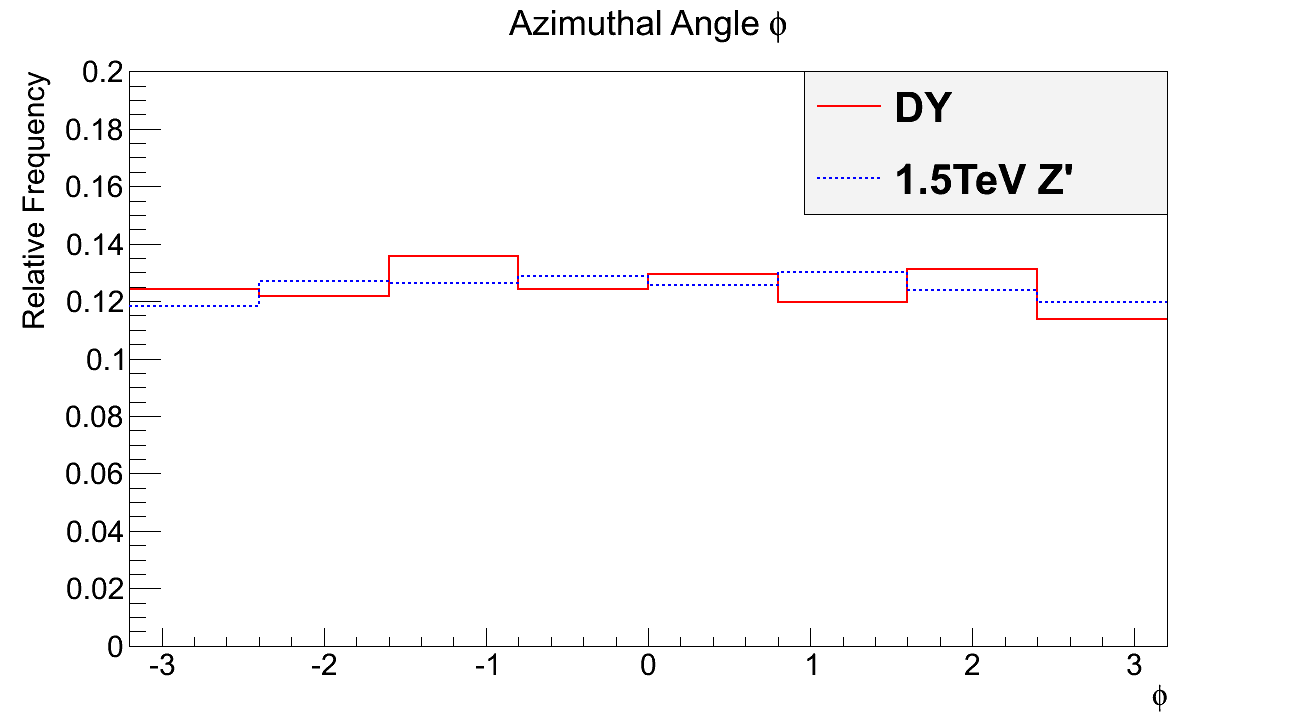
\includegraphics[height=0.6\textwidth]{images/variables/Phi.png}
        \caption{}
        \label{fig:phi}
    \end{subfigure}
    \begin{subfigure}{.49\textwidth}
        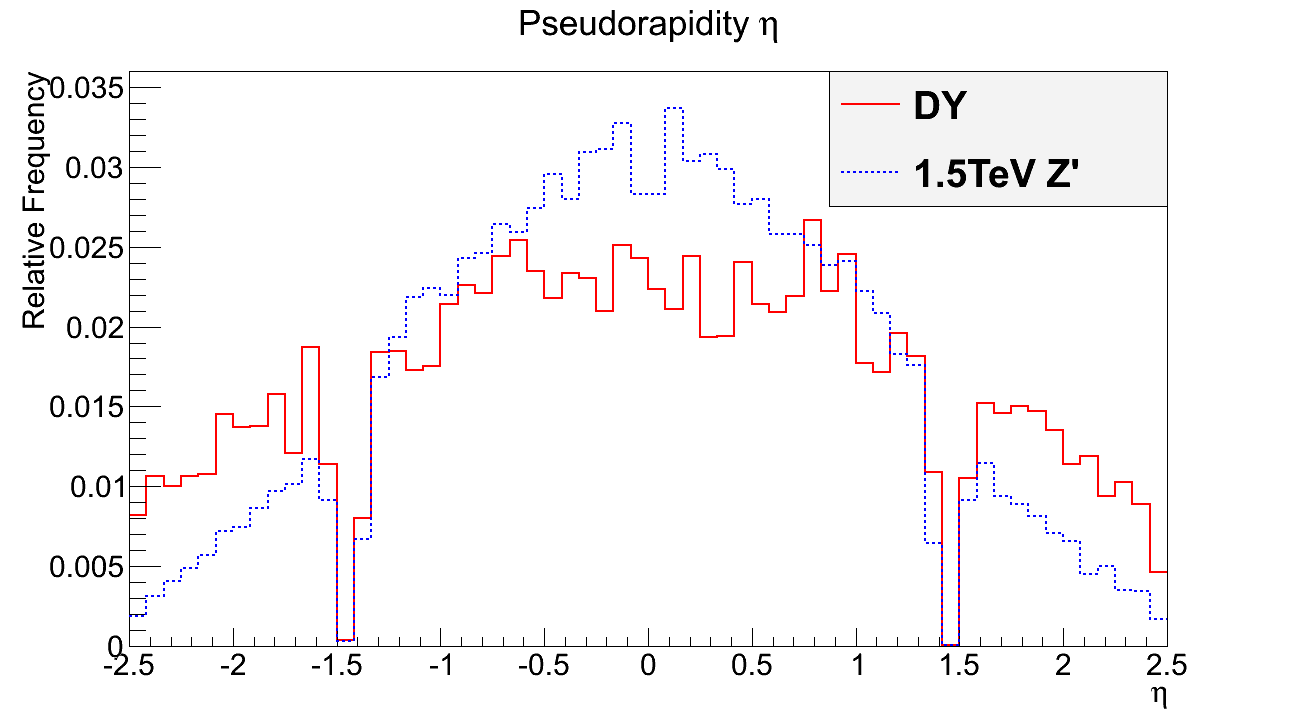
\includegraphics[height=0.6\textwidth]{images/variables/Eta.png}
        \caption{}
        \label{fig:eta}
    \end{subfigure}
    \caption{\label{fig:etaPhi}}
\end{figure}

In Figure \ref{fig:phi}, the distribution of the azimuthal angle of final state particles is seen to be relatively uniform. This is consistent with what would be expected as the total longtitudinal momentum is zero, meaning that the angular distribution in this plane should be uniform as well. The pseudorapidity of Drell-Yan and $Z'$ events is shown in Figure \ref{fig:eta}. From this, it can be seen that the $Z'$ final states are more central than Drell-Yan events. This is due to the $1.5\,$TeV $Z'$ states having a larger invariant mass than most of the Drell-Yan dilepton pairs. No linear cuts are placed on $\phi$ and $\eta$ due to the similarity between signal and background distributions.

\subsubsection{$R_{\eta}$ and $R_{\phi}$}

The parameters $R_{\eta}$ and $R_{\phi}$ are related to the cluster energies contained in a region of interest in the detector cells. $R_{\eta}$ corresponds to the ratio of the energy in the $3\times7$ cell region to the $7\times7$ region centered at the cluster position. Conversely, $R_{\phi}$ is equal to the ratio of the energy in the $3\times3$ region to the $3\times7$ region. These quantities relate to the width and height of the cone respectively. If the ratios are close to one, this indicates the majority of the cone's energy is focused in the centre of the cluster.

The distributions for $R_{\eta}$ and $R_{\phi}$ can be seen in Figures \ref{fig:rEta} and \ref{fig:rPhi} respectively. As the $Z'$ distributions in $R_{\eta}$ and $R_{\phi}$ are centred closer to 1, it can be inferred that the cluster energy is more tightly focused in the centre for the $Z'$ than the other samples. Minimum cuts were placed at $0.95$ and $0.96$ for $R_{\eta}$ and $R_{\phi}$ respectively.

\begin{figure}[h]
    \centering
    \begin{subfigure}{.49\textwidth}
        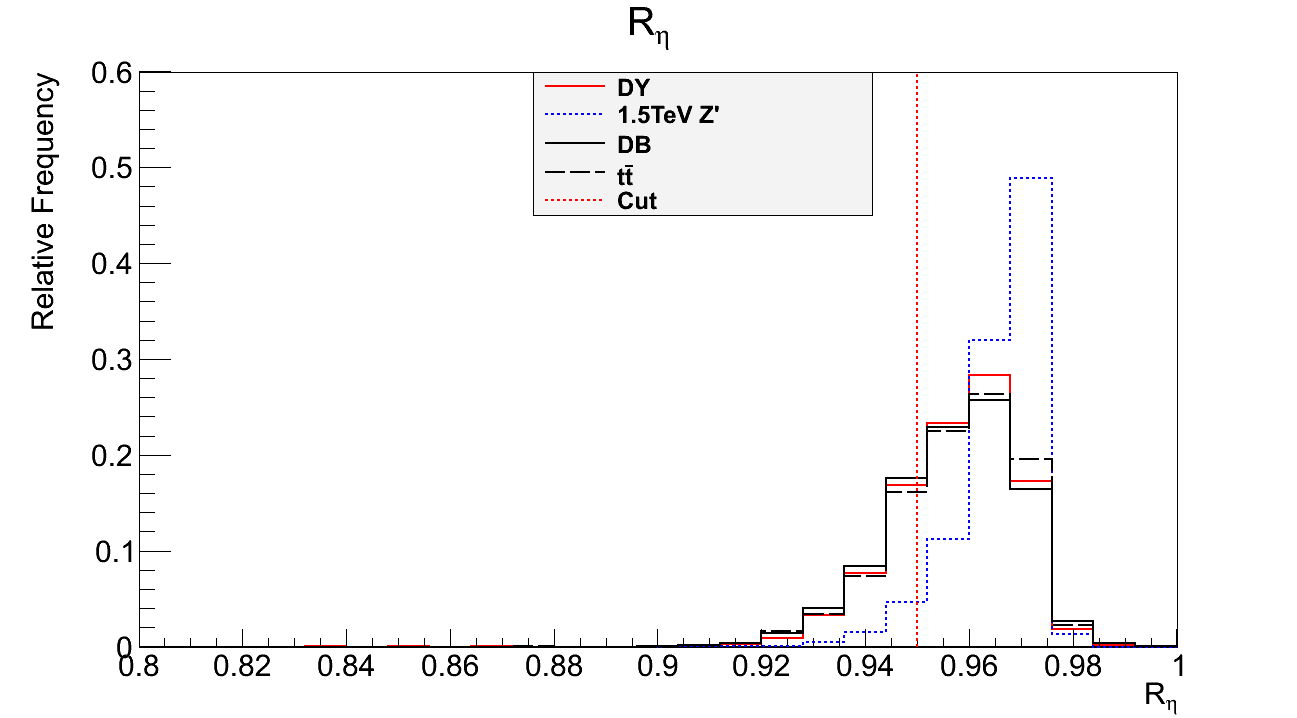
\includegraphics[height=0.6\textwidth]{images/variables/rEta.png}
        \caption{}
        \label{fig:rEta}
    \end{subfigure}
    \begin{subfigure}{.49\textwidth}
        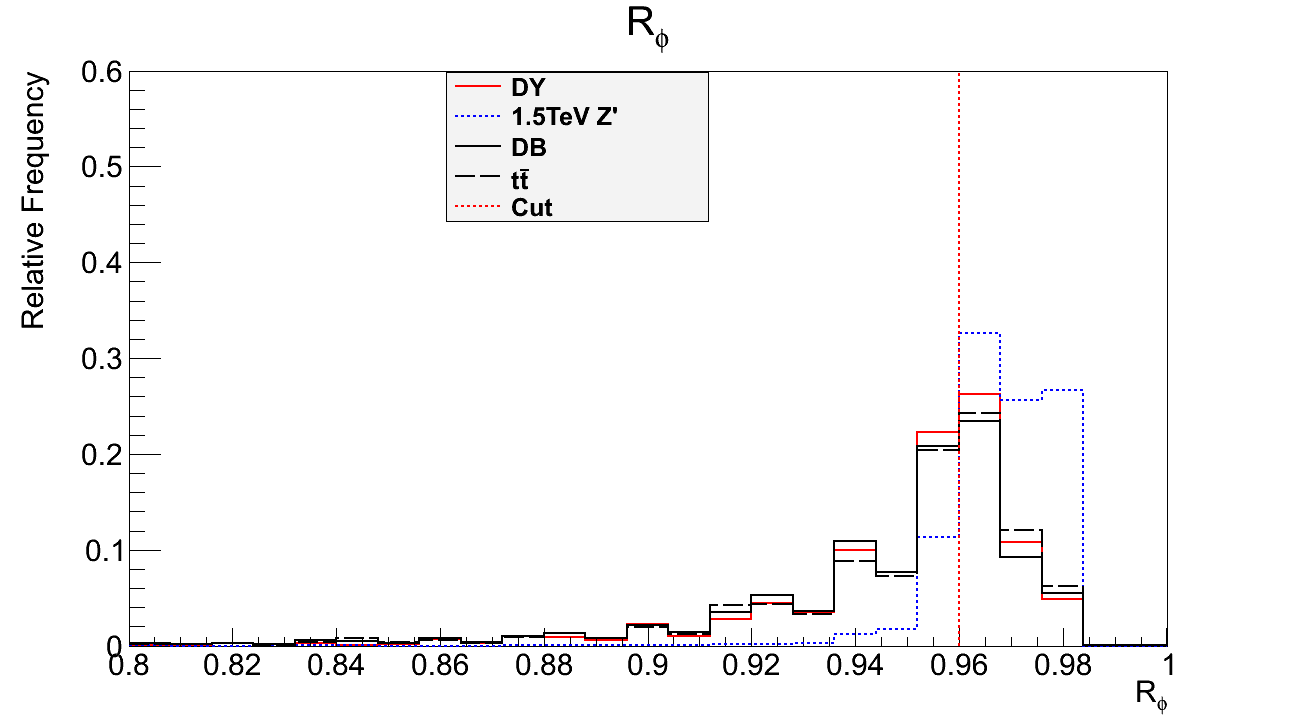
\includegraphics[height=0.6\textwidth]{images/variables/rPhi.png}
        \caption{}
        \label{fig:rPhi}
    \end{subfigure}
    \caption{ (a) $R_{\eta}$, the ratio of the energy in the $3\times7$ region over the energy in the $7\times7$ cell region centered at the cluster position, is plotted. The dashed line shows the minimum cut value, which is set at $0.95$. (b) $R_{\phi}$, the ratio of the energy in the $3\times3$ region over the energy in the $3\times7$ cell region centered at the cluster position, is also shown. The minimum cut is placed at $0.96$. \label{fig:rEtaRPhi}}
\end{figure}


\subsubsection{Lateral Width, $W_{\eta^2}$}

The lateral width

\begin{figure}[h]
    \centering
    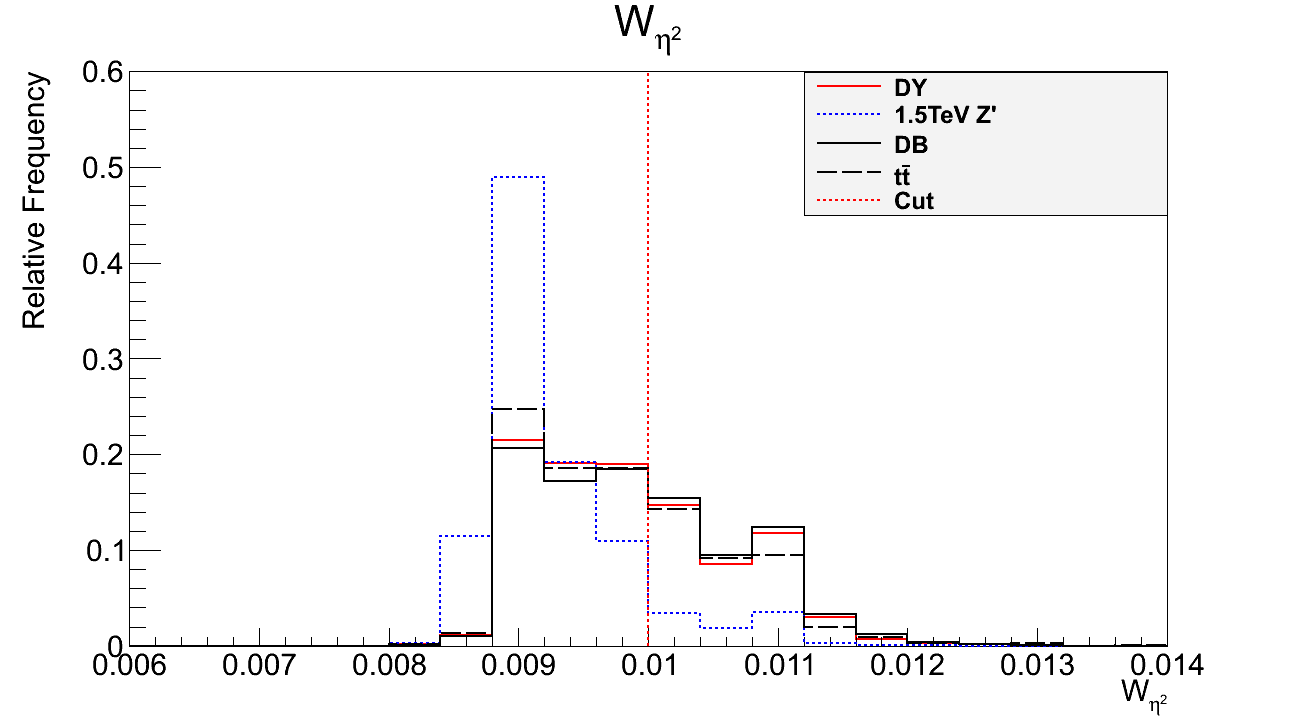
\includegraphics[scale=0.25]{images/variables/wEta.png}
    \caption{$W_{\eta^2}$, the lateral width of the shower, is plotted. The dashed line shows the maximum cut value, which is set at $0.01$\label{fig:wEta}. }
\end{figure}


\subsubsection{Efficiency of Cuts}

The overall linear cuts identified in this section are listed in Table [TODO].

\begin{table}[h!t]
\centering
\caption{ Variables Associated with the medium selection criteria \cite{ElectronPerformanceMeasurements}\label{table:mediumVariables}}
\begin{tabular}{|c|c|c| } 
\hline
Variable & Minimum Cut & Maximum Cut\\\hline
$E_T$ & $200\,$GeV  & -\\\hline
$R_{\eta}$ & $0.95$ & -\\\hline
$R_{\phi}$ & $0.96$ & -\\\hline
$W_{\eta^2}$ & - & $0.01$ \\\hline
\end{tabular}
\end{table}


\subsection{Detector Resolution Study}

%http://inspirehep.net/record/796888?ln=en

The acheivable energy resolution of the $Z'$ mass was investigated using the Monte Carlo dataset. The energy resolution of a simulated $Z'$ event is obtained using the reconstructed $Z'$ mass $M_{Z'}$ and the true mass of the simulated $Z'$ before it is ``smeared'' in the simulation, $M_{\rm{Truth}}$, by the equation

\begin{equation}
\frac{\Delta M_{Z'}}{\Delta M_{\rm{Truth}}} = \frac{M_{\rm{Recon}}-M_{\rm{Truth}}}{M_{\rm{Truth}}}.
\end{equation}

As the true mass is not stored in the Monte Carlo event data but rather the true transverse momenta, energy and coordinates, the true mass of  the simulated $Z'$ is reconstructed using the equations for the momentum components

\begin{equation}
\begin{split}
P_x & = P_T \cos\phi \\
P_y & = P_T \sin\phi \\
P_z & = P_T\sinh\eta \\
\end{split}
\end{equation}

and the equation for the invariant mass of the particle

\begin{equation}
M^2 = \left(\sum E\right)^2 - \left(\sum \bf{P}_i\right)^2,
\end{equation}

where here natural units are adopted and $c$ is set to 1. 

It is shown in \cite{ATLASResolutionEquation} that the energy resolution for measurement of the invariant mass of an electron pair can be modelled as an equation of the form

\begin{equation}
\frac{\sigma(E)}{E} = \frac{a}{\sqrt{E}} \oplus \frac{b}{E} \oplus c,
\end{equation}

where $a$ and $b$ are stochastic and noise terms respectively.

\begin{figure}[h]
    \centering 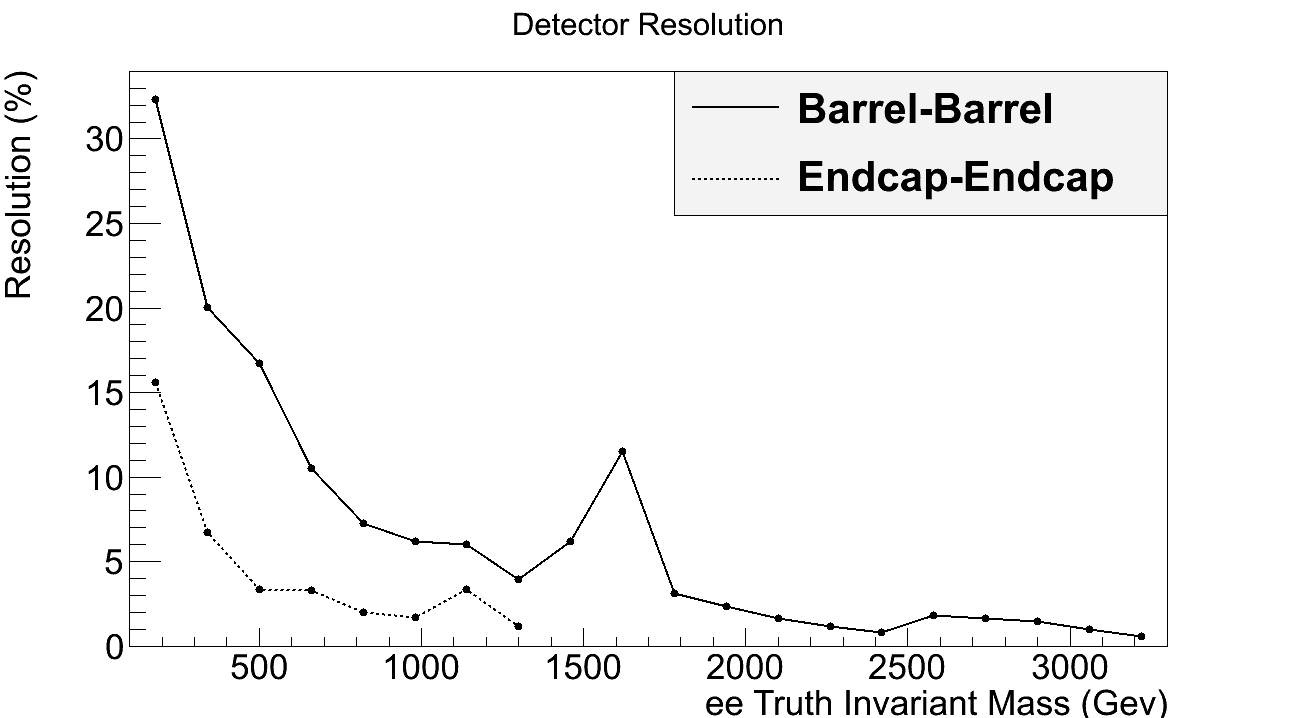
\includegraphics[scale=0.3]{images/resolution.png} \caption{ The resolution of the detector in both the barrel and endcap regions is  is plotted.  \label{fig:Resolution}.}
\end{figure}

The resolution of the detector, $\sigma_{\rm{det}}$, is plotted as a function of the invariant mass of a reconstructed particle in Figure \ref{fig:Resolution}. Drell-Yan samples are used here as the process is very similar kinematically to that of the $Z'$, and is a larger sample than that available in the $Z'$ data set, improving the uncertainty associated with the measurement of the resolution. The Drell-Yan set also exists over a larger range, allowing the evolution of the resolution of the detector as a function of the invariant mass to be investigated. It is seen that for both the barrel and endcap regions, the resolution tends towards $1\%$ at higher energies, of the order of $2\,$TeV. However, in the low energy range the uncertainty in the measurement of the invariant mass is significantly higher than expected.

\subsection{Trigger and ID Criteria Efficiencies}
\begin{figure}[h]
    \centering 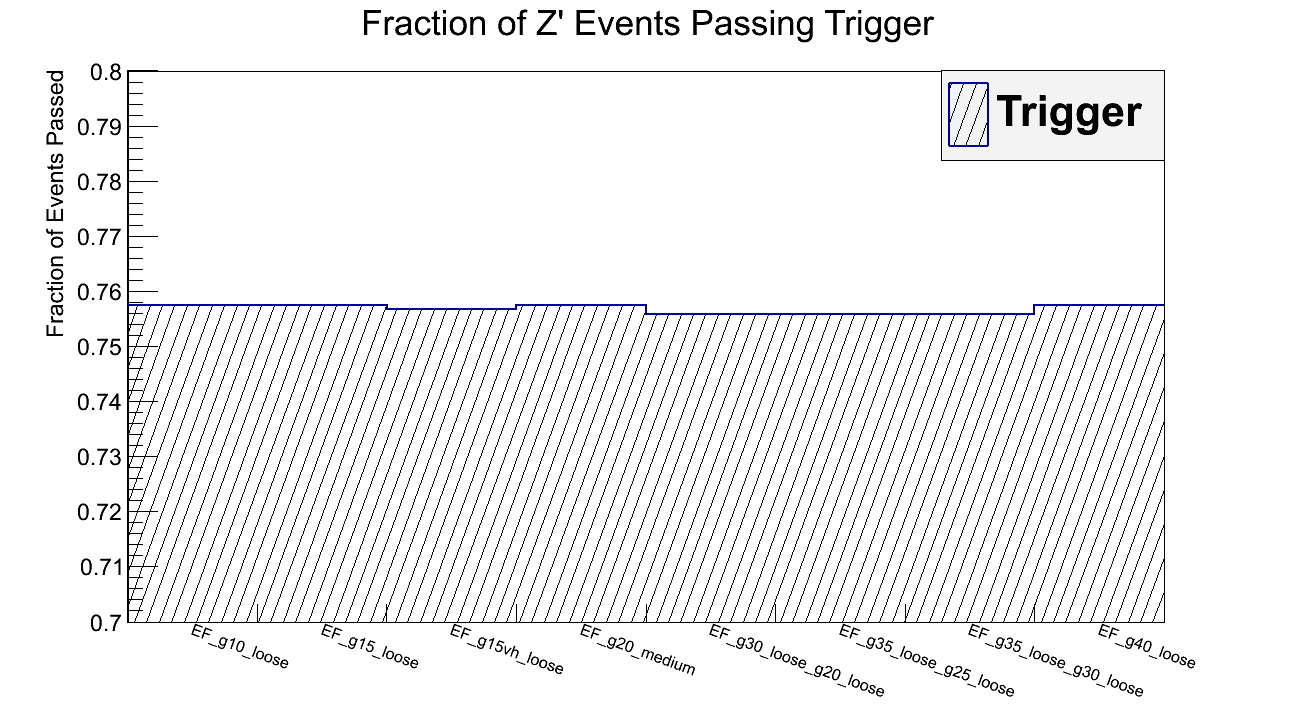
\includegraphics[scale=0.3]{images/TriggerZ.png} \caption{ The fraction of signal events passing the trigger \label{fig:TriggerZ} }
\end{figure}

\subsection{Barrel and Endcap}

In the experiment, it is useful to determine the likely position of the final state pairs in the detector. The positions of the dilepton pair can be categorised as one of three combinations; these are barrel-barrel, barrel-endcap, and endcap-endcap. As the name suggests, a barrel-barrel event is one in which both final state leptons are located in the barrel of the EM calorimeter (TODO: or inner detector?), while barrel-endcap events are those in which one lepton is located in the barrel and another in the endcap. As discussed in Section \ref{sec:ATLAS_DetectorSchematics}, an electron is located in the barrel if its pseudorapidity $|\eta|<1.37$. If $|\eta|>1.52$ the lepton is located in the endcap, with leptons located in the crack region between the two not passing the selection criteria.

\begin{figure}[htb]
	%\centering
    \begin{subfigure}{.5\textwidth}
        \raggedleft
        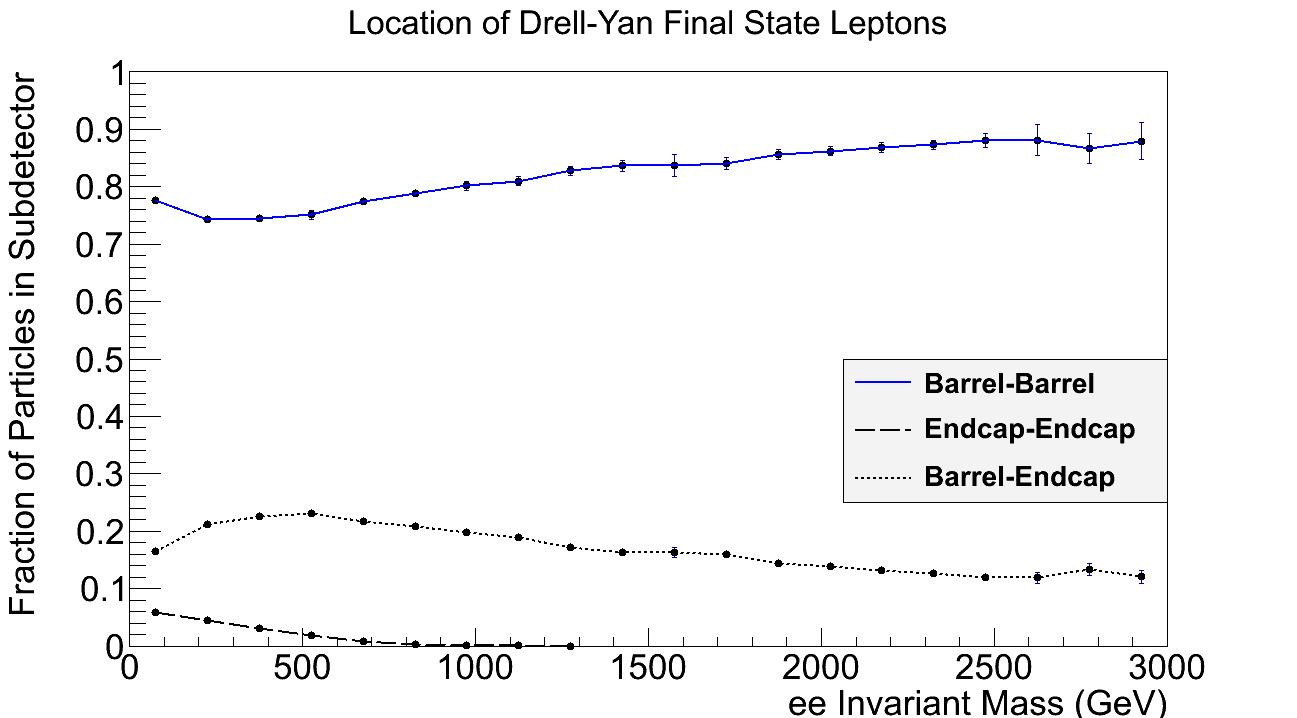
\includegraphics[width=\textwidth]{images/barrelEndcapDY.png}
        \caption{}
        \label{fig:BEDY}
    \end{subfigure}
    \begin{subfigure}{.5\textwidth}
       	\raggedright
        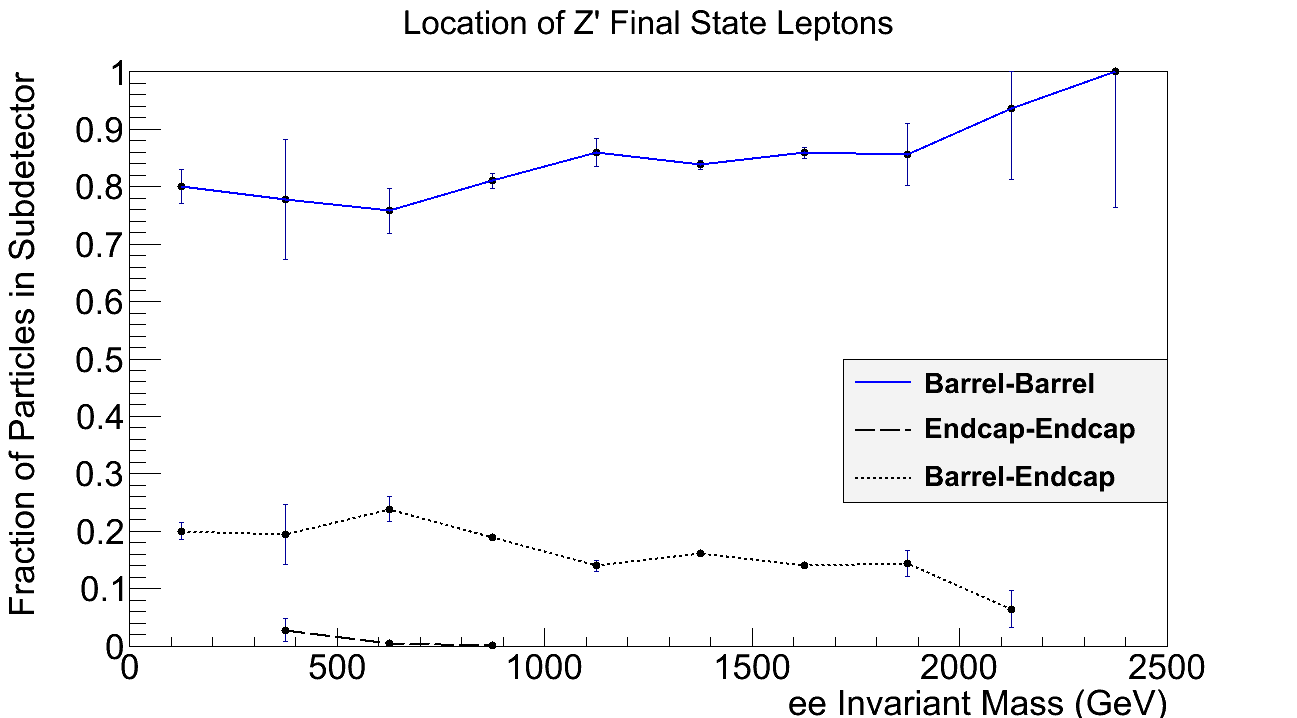
\includegraphics[width=\textwidth]{images/barrelEndcapZ.png}
        \caption{}
        \label{fig:BEZ}
    \end{subfigure}	
    \caption{The fraction of barrel-barrel, endcap-endcap and barrel-endcap final state pairs are plotted as a function of the ee invariant mass for (a) Drell-Yan leptons and (b) a $1.5\,$TeV $Z'$. A smaller number of bins are used for the $Z'$ due to the smaller number of events available in the sample.\label{fig:BarrelEndcap}}
\end{figure}

The fraction of events falling into this category are plotted for the Drell-Yan sample and the $1.5\,$TeV $Z'$ sample. It can be seen that in the TeV range, in which  a $Z'$ may be located, more than $80\%$ of dilepton pairs fall in to the `barrel-barrel' category. 

\subsection{Forwards Backwards Asymmmetry}

Forwards backwards asymmetry defined as 
\begin{equation}
\rm{Asym} = \frac{n_f - n_b}{n_f + n_b}
\end{equation}
The quantity $\theta^*$ represents the polar angle $\theta$ between the $x-y$ plane and a final state electron in the reference frame of the other electron.
\begin{figure}[h]
    \centering 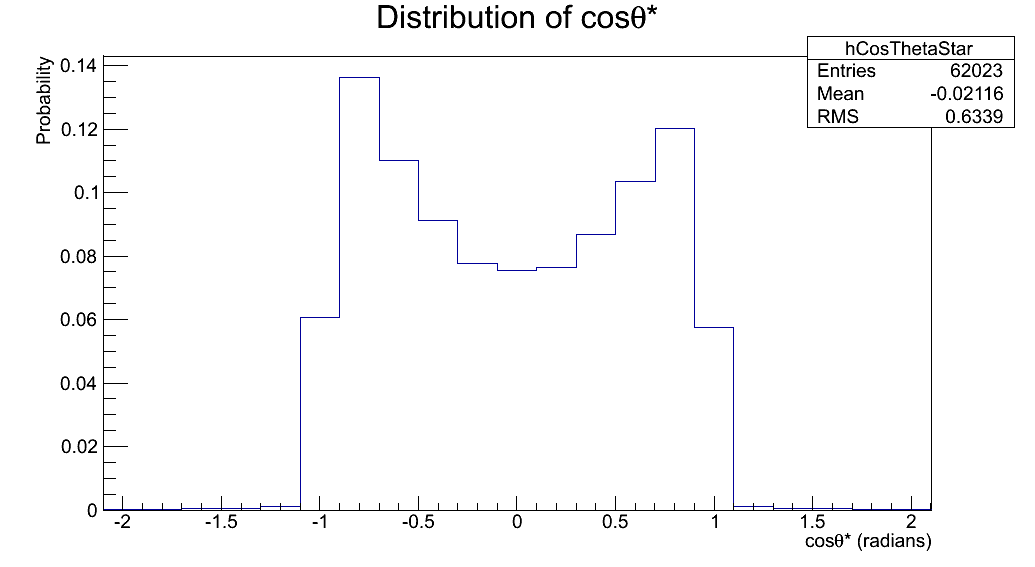
\includegraphics[scale=0.3]{images/cosThetaStar.png} \caption{The probability as a function of $\cos\theta^*$ for Drell-Yan final state electrons is plotted. A slight backwards asymmetry can be seen. \label{fig:cosTheta} }
\end{figure}

\section{Conclusion}
\label{sec:Conclusion}

\section{Appendix}
\subsection{Asimov Significance Errors}
\label{sec:appendix_errors}
For a multivariate function $f$ depending on a set of variables $\overrightarrow{x}$, the resultant uncertainty in $f$ can be expressed as 
\begin{equation}
\Delta f(\overrightarrow{x}) = \sqrt{\sum_{i=1}^{n} 
\left( \frac{\partial f}{\partial x_i}\Delta x_i \right)^2}
\end{equation}

For the approximate discovery significance $\frac{s}{\sqrt{b}}$, the error in this statistic is given by

\begin{equation}
\sqrt{\left( \frac{\Delta s}{\sqrt{b}} \right)^2 + \left( \frac{s\Delta b}{-2x^{-3/2}} \right)^2 } = \sqrt{\frac{(\Delta s)^2}{b} + \frac{s^2 (\Delta b)^2}{4b^{3}}}
\end{equation}

\subsection{Type I and II errors}

In practise, there always exists some probability of rejecting the null hypothesis $H_0$ in favour of the signal hypothesis $H_1$. This is known as a type I error and its probability $\alpha$ is given by the equation
\begin{equation}
\alpha = \int_{W}f(x|H_0)dx,
\end{equation}
where $W$ is the signal region and $f(x|H_0)$ is the background probability density function. This is also known as the false discovery rate or significance.

Conversely, type II errors are defined as accepting the null hypothesis if $H_1$ is true. Its probability is equal to
\begin{equation}
\beta = \int_{W}f(x|H_1)dx.
\end{equation}
The power of the test with respect to the hypothesis $H_1$, or the probability of accepting $H_1$ when it is true is equal to $1-\beta$.

From Bayes' theorem, the posterior probability the signal purity is given by
\begin{equation}
P(s|x\in W) = \frac{P(x\in W|s)P(s)}{P(x\in W|s)P(s) + P(x \in W|b)P(b)}
\end{equation}

here $W$ is the signal region and $P(s)$ is the prior probability. $P(x\in W|s) = \epsilon_{\rm{s}}$, where $\epsilon_{\rm{s}}$ is known as the signal efficiency- this is equivalent to the power of the experiment $1-\beta$. Conversely, $P(x \in W|b) =  \int_{W}f(x|H_0)dx = \epsilon_{\rm{b}}$, where $\epsilon_{\rm{b}}$ is the background efficiency, equal to the significance $\alpha$.

\subsection{Neyman-Pearson Lemma}
In order to optimise the critical region, the boundary at which a transverse energy cut is applied, the Neyman-Pearson lemma \cite{NeymanPearsonLemma} is applied. This requires that the test statistic

\begin{equation}
t(x) = \frac{f(x|H_1)}{f(x|H_0)}
\end{equation}

is maximised, where $f(x|H_1)$ and $f(x|H_0)$ are the probability density functions for $Z'$ and $DY$ events in this case.

\subsection{Cross Sections}

\begin{table}[h!t]
\label{table:DYXS}
\centering
\caption{ Drell-Yan cross sections }
\begin{tabular}{ |c|c| } 
\hline
Mass (GeV) & $\sigma B\,$(fb)\\\hline
$120-180$ & $9846$ \\\hline
$180-250$ & $1571$\\\hline
$250-400$ & $549.2$\\\hline
$400-600$ & $89.66$\\\hline
$600-800$ & $15.1$\\\hline
$800-1000$ & $3.75$\\\hline
$1000-1250$ & $1.293$\\\hline
$1250-1500$ & $0.3577$\\\hline
$1500-1750$ & $0.1123$\\\hline
$1750-2000$ & $0.03838$\\\hline
$2000-2250$ & $0.01389$\\\hline
$2250-2500$ & $5.23\times10^{-3}$\\\hline
$2500-2750$ & $2.02\times10^{-3}$\\\hline
$2750-3000$ & $7.89\times10^{-4}$\\\hline
$3000+$ & $5.04\times10^{-4}$\\\hline
\end{tabular}
\end{table}

%http://w3.iihe.ac.be/~bclerbau/Summer07/cross_section_BSM.text
\begin{table}[h!t]
\label{table:ZPrimeXS}
\centering
\caption{ $Z'$ cross sections }
\begin{tabular}{ |c|c| } 
\hline
Mass (GeV) & $\sigma B\,$(fb) \\\hline
$1500$ & $15.134$ \\\hline
$2000$ & $2.556$ \\\hline 
$2500$ & $0.696$ \\\hline
\end{tabular}
\end{table}

\begin{table}[h!t]
\label{table:DBi}
\centering
\caption{ Diboson cross sections }
\begin{tabular}{ |c|c| } 
\hline
Process & $\sigma B\,$(fb) \\\hline
$WW$ & $1.149\times10^4$ \\\hline
$WZ$ & $3481$ \\\hline 
$ZZ$ & $976$ \\\hline
$t\overline{t}$ & $8.02\times10^4$\\\hline
\end{tabular}
\end{table}

\subsection{Asimov Partial Derivatives}

Using the chain rule, the rate of change of discovery significance with respect to the search window size can be expressed as

\begin{equation}
\frac{d Z_0}{d W} = \frac{\partial Z_0}{\partial s}\frac{\partial s}{\partial W} + \frac{\partial Z_0}{\partial b}\frac{\partial b}{\partial W} = 0.
\end{equation}

The partial derivatives of Equation \ref{eqn:asimov} are equal to

\begin{equation}
\begin{split}
\frac{\partial Z_0}{\partial s} & = \frac{\ln(\frac{s}{b}+1)}{\sqrt{2\left((b+s)\ln(\frac{s}{b}+1))-s\right)}} \\ 
\frac{\partial Z_0}{\partial b} & = \frac{\ln(\frac{s}{b}+1)-\frac{s}{b}}{\sqrt{2\left((b+s)\ln(\frac{s}{b}+1))-s\right)}}.
\end{split}
\end{equation}
\bibliographystyle{unsrt}
\bibliography{./references}
\end{document}